\documentclass{article}
 
\usepackage[margin=1in]{geometry}
\usepackage[strict]{changepage}
\usepackage{float}
\usepackage{fancyhdr}
\usepackage{mhchem}
\usepackage{siunitx}
\usepackage{wrapfig, booktabs}
\usepackage{enumitem}
\usepackage{ctex}
\usepackage{graphicx}
\usepackage{amsmath}
\usepackage{amssymb}
\usepackage{subfigure}
\usepackage{multirow}
\usepackage{multicol}
\usepackage{wrapfig}
\usepackage{indentfirst}
\usepackage[utf8]{inputenc}
\usepackage{geometry}
\usepackage{setspace}   %set space between lines
\usepackage{graphicx} %insert figure 
\usepackage{float} %设置图片浮动位置的宏包
\usepackage{subfigure} %插入多图时用子图显示的宏包
\usepackage{listings}   %插入代码的宏包
\usepackage{xcolor} % to define color 
\usepackage{verbatim}   %for comment 
\usepackage[breaklinks,colorlinks,linkcolor=black,citecolor=black,urlcolor=black]{hyperref} %for bookmark 



\setlength{\parindent}{2em}

\definecolor{mygray}{rgb}{0.5,0.5,0.5}  %totally used in code display
\definecolor{mygreen}{rgb}{0,0.6,0}

\lstset{                %代码显示格式设置
    numbers=left,                                   
    % where to put the line-numbers; possible values are (none, left, right)
    numberstyle=  \color{mygray}, 
    % the style that is used for the line-numbers
    keywordstyle= \color{ blue!70},
    basicstyle=\footnotesize,        
    % the size of the fonts that are used for the code
    commentstyle=\color{mygreen},    
    % comment style
    frame=single,	                   
    % adds a frame around the code, you can use frame=shadowboxs
    % with a rulesepcolor= \color{ red!20!green!20!blue!20} ,
    escapeinside=``, % 英文分号中可写入中文
    xleftmargin=4em,xrightmargin=2em, aboveskip=1em,
    framexleftmargin=2em
} 


\begin{document}

\begin{spacing}{1.5}

    %title  page 
    \thispagestyle{empty}
    \begin{center}
~\\[6cm]\rule{\linewidth}{0.5mm} \\[6mm]
{\Large 综合论文  \\  \textbf{{\LARGE 智能风扇}}  \\[6mm]}
\rule{\linewidth}{0.5mm} \\[2cm]
{\Large 姓 名: 吕光冉}\\[.3cm]
{\Large 班 级:   自73 }\\[.3cm]
{\Large 学 号:  2017011574}\\[.3cm]
{\Large 日 期:\today }\\[.3cm]
    \end{center}

    \clearpage
    \phantom{s}

    %if need to make table of contents in pdf, below command is okay
\tableofcontents
\newpage

    \subsection{摘要}

    本文介绍了一个智能风扇系统的设计与实现。本设计以Arduino Mega为主控板,利用基于PT1000的灵敏
    温度测量电路感知环境温度,利用基于热释电传感探头RE200B的人体感知电路感知人是否在检测范围内出现,
    利用这两个方面的环境信息来自动调整风扇转速。同时,为了实现风扇的可携带性,本设计在电源管理模块中,
    使用了5V电压稳压可调节模块,正负电源模块和DC/DC升压斩波电路等模块来配合12V锂电池来给电路提供电源。

    \textbf{关键词} :智能风扇;小型电子系统设计;模拟电路;数字电路

\section{引言}

   我所选择的第二个综合论文题目为智能风扇系统的设计与制作。
    
   在炎炎夏日,一个好的可携带风扇对人们就变得十分重要。在我自己使用风扇的过程中,我发现
   市面上所售卖的风扇主要存在以下两个问题:一方面,如果忘记关闭风扇电源,即使是在人已经离开房间
   以后,它也不能自动关闭以节省电池电量,另一方面,大多数风扇都不具备测温功能,只能通过用户手动根据体感温度
   调节风扇转速。

    所以说,我想要自己设计并实现这样一款智能风扇:一,它首先要体积较小,使用电池供电,具有可携带性;二,
    它要能够感知人体,在人离开风扇的检测距离以后,自动关闭风扇;三,它应该能够根据环境温度,智能调节风扇
    转速;四,它最好能实现比较好的用户互动,有显示屏和蓝牙APP等方式来接收用户指令。

\section{设计目标}

\begin{enumerate}
    \item 使用电池供电,具有便携性
    \item 能进行人体检测,在人离开检测范围后,关闭风扇
    \item 能根据环境温度,智能调节风扇转速
    \item 有显示屏显示当前工作状态
    \item 能通过蓝牙进行连接,与用户手机APP进行连接后,由用户调节其在不同温度下的转速
\end{enumerate}

\section{实现方式}

整个电子系统的实现框图如图\ref{fig:design_total}所示:

\begin{figure}[H]
    \centering
    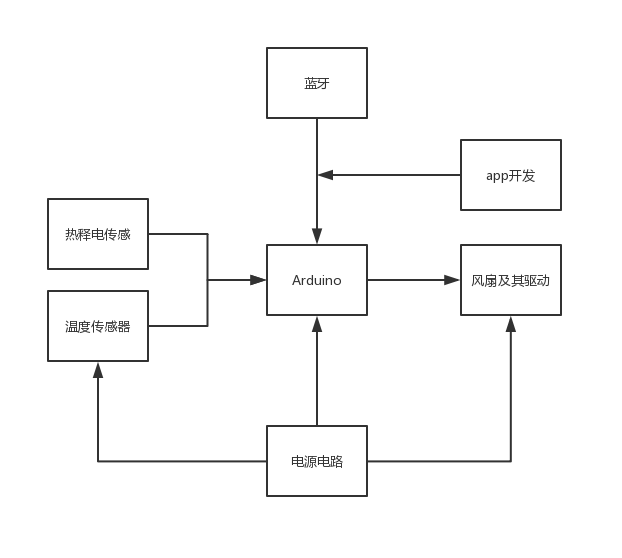
\includegraphics[scale=0.4]{fig/design/total.png}
    \caption{整体电路实现框图}
    \label{fig:design_total}
\end{figure}

在这里,我将整个电子系统分为下列模块:主控板模块,温度传感器模块,热释电传感模块,风扇及其驱动模块,蓝牙模块与对应
的APP,电源电路模块。

其中,热释电传感器是用来实现人体检测的功能,
温度传感器负责检测环境温度,
风扇及其驱动电路负责驱动风扇运转,
蓝牙及APP模块负责实现与用户的蓝牙连接,
主控板Arduino Mega负责实现数字控制逻辑,
即获取热释电传感和温度传感器输出的环境信息,
根据用户蓝牙设置的预定义功能,
自主决定风扇转速。
并且,整个电路的供电问题,都由电源管理模块负责。

其中,根据传感器,主控板,风扇等模块所需要的电源类型,电源管理模块
包括有:

\begin{figure}[H]
    \centering
    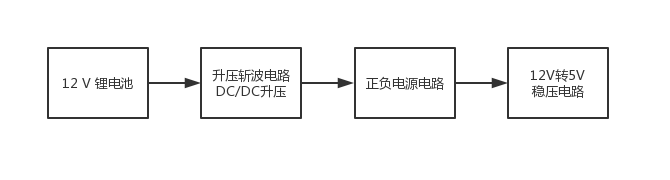
\includegraphics[scale=0.4]{fig/design/total1.png}
    \caption{电源管理模块设计}
    \label{fig:design_total1}
\end{figure}

而整个项目我的基本调试流程如下:

\begin{figure}[H]
    \centering
    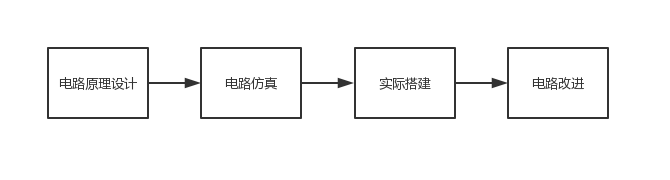
\includegraphics[scale=0.4]{fig/design/flow.png}
    \caption{基本调试流程}
    \label{fig:design_flow}
\end{figure}

在下文中,我也将根据这一思路,阐述我的电路的设计过程,仿真结果以及实测结果。

 
\section{基本电路模块电路原理}

    \subsection{模拟电路模块}

    \begin{enumerate}
        \item 5V稳压电路
        
        5V稳压电路电路原理图:

        \begin{figure}[H]
            \centering
            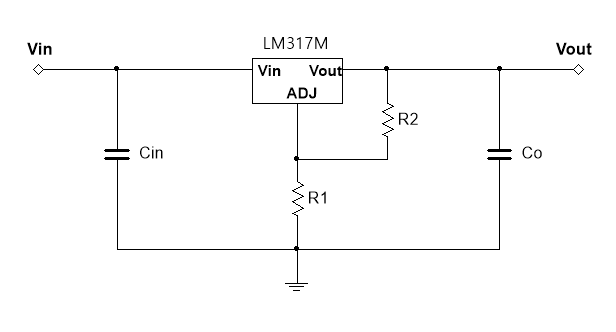
\includegraphics[scale=0.4]{fig/design/principle1.png}
            \caption{5V稳压电路原理图}
            \label{fig:design_prin_1}
        \end{figure}
        
        我为了实现5V电压可以进行微调,使用了一个电压可调电路。其中,三端稳压器使用了
        LM317M。在输入电压足够大,公共端ADJ处电流可以近似忽略的条件下,电路输出电压满足关系:

        \begin{equation}
            V_{out} = 1.25(1+\frac{R_2}{R_1}) V
        \end{equation}

        由于使用到了三端稳压器,其脉动系数 S 应该不会太大,可以满足后级电路需求。

        \item 正负电源电路
        
        我设计的正负电源电路原理图如图\ref{fig:design_prin_2}所示:
        \begin{figure}[H]
            \centering
            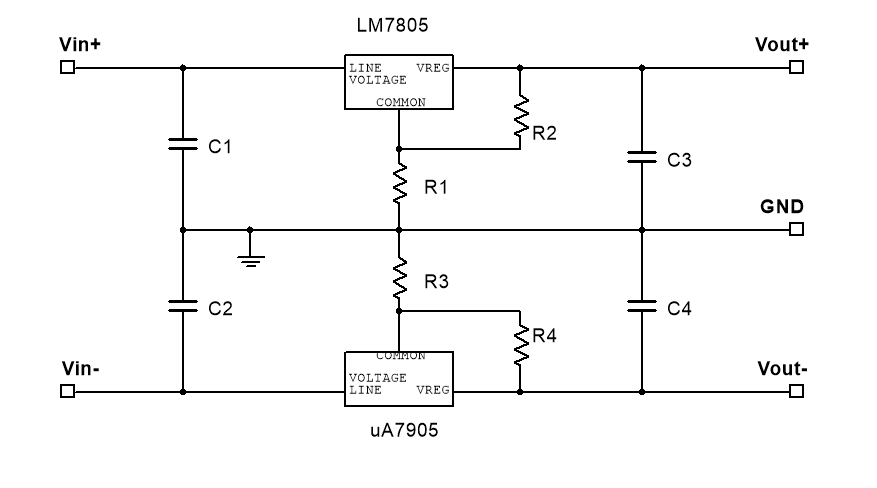
\includegraphics[scale=0.4]{fig/design/principle2.png}
            \caption{正负电源电路}
            \label{fig:design_prin_2}
        \end{figure}
        
        在输入电压足够大,并且COMMON端电流可以被近似忽略时,电路输出近似满足下列关系:
        \begin{equation}
            \begin{cases}
                V_{out+} = 5(1+\frac{R_1}{R_2}) V \\
                V_{out-} = -5(1+\frac{R_3}{R_4}) V
            \end{cases}
        \end{equation}

        \item 温度测量电路
        
        温度测量电路原理图如图\ref{fig:design_prin_3}所示:

        \begin{figure}[H]
            \centering
            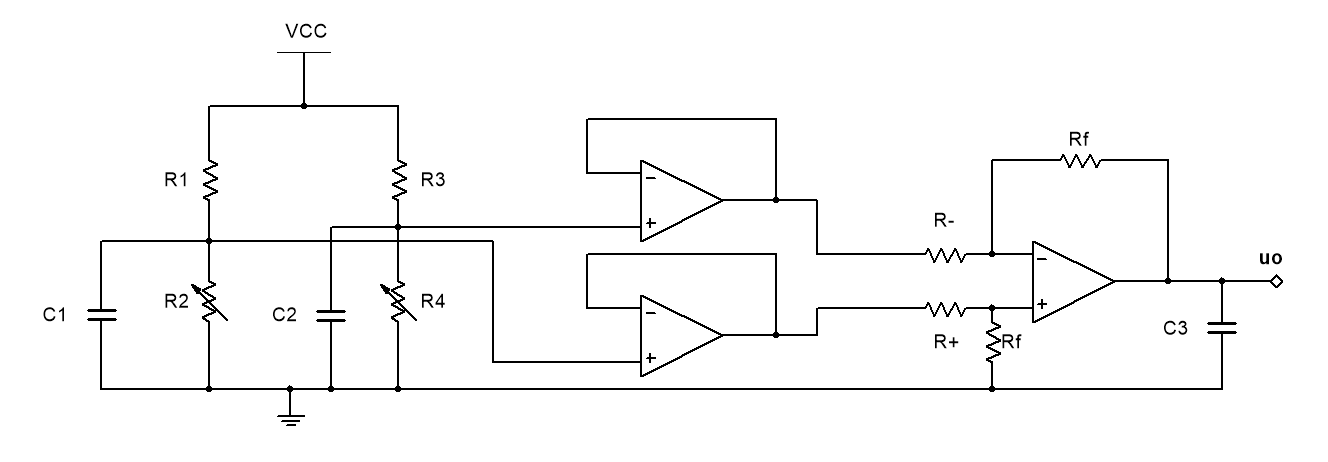
\includegraphics[scale=0.4]{fig/design/principle3.png}
            \caption{温度测量电路原理图}
            \label{fig:design_prin_3}
        \end{figure}

        温度测量电路的设计是基于铂电阻(PT1000)的温度特性。铂电阻在不同温度下的阻值不同且数值比较固定,
        在将铂电阻阻值变化转变为电信号后,经过一定的运算电路就可以得到比较精确的温度测量值。

        在电路图中,$R_2$ 为 PT1000 铂电阻,其阻值随温度变化,$R_4$ 为调零电阻,可以调整电路使其在0$^{\circ}C$ 
        时输出为0。
        R1,R2,R3,R4构成电桥电路。电桥电路的两个输出值
        在经过由精密运放构成的跟随器之后,
        进入最后一级电路做差并被放大。
        原理图中C1,C2负责稳定输入电压,消除自激振荡,
        C3负责稳定输出电压,滤去高频噪声。
        
        根据 PT1000 铂电阻的温度特性,在0摄氏度时,PT1000电阻阻值为1000 $\Omega$,其后,每上升1摄氏度,
        其阻值大致上升4 $\Omega$. 则根据R1,R2分压关系,可知在 k 摄氏度时,如果假设$R_1$足够大,则电桥左路的输出电压为:

        \begin{equation}
            V_{+} = \frac{R_2}{R_2 + R_1} V_{CC} = \frac{1000+4k}{R_1 + 1000 + 4k} V_{CC} \approx \frac{1000+4k}{R_1 + 1000 } V_{CC} \label{equ:approx}
        \end{equation}

        此时,若调节电路在0摄氏度时输出为0,则电桥右路输出电压为:
        \begin{equation}
            V_{-} = \frac{R_4}{R_3 + R_4} V_{CC} = \frac{1000}{1000 + R_1 } V_{CC}
        \end{equation}

        因此,在最后一级,当正极输入电阻和输出电阻阻值相等时,有:
        \begin{equation}
            V_{out} = \frac{R_f}{R_{+}} (V_{+} - V_{-}) \approx \frac{R_f}{R_{+}} \cdot \frac{4k}{R_1 + 1000} V_{CC}  
        \end{equation}

        通过最后一级的比例调整,将电压近似的转化为主控板可以直接读取的模拟电压值。

        \item 热释电测量电路
        
        热释电传感电路用于检测指定距离内是否有人存在。其基本测量原理是热释电基于热释电传感探头(三极管)的三端特性。
        热释电传感探头可以将吸收到的红外辐射转化为微弱的电信号,而在热释电探头上加上菲涅尔透镜则可以有效削弱环境干扰信号,
        保留人体热电信号,所以该传感探头可以用于测量是否有人在其探测范围内。

        但是经过测量,我发现,我们使用的被动式热释电传感探头实际上并不完全可靠。当有人进入探头的探测范围(由于项目需要,
        我设定为20cm)后,热释电传感探头输出电平是一个直流分量和近似为RC衰减分量的叠加。其中,直流分量数值不确定,会随着环境光强
        的变化而变化;RC衰减分量表现为短时间内电平下降0.2V,然后逐渐恢复至0。
        
        同理,在人离开探头的探测范围后,热释电传感探头输出端会有一个大约为0.1V左右的压升,
        然后电平仍然会基本类似于RC衰减,缓慢回到原来的电压水平。

        根据热释电传感探头的工作原理,我一共设计了两版热传感电路,其工作原理都是基于检测传感器是否有电平变化来判断
        是否有人进出传感探头检测范围,并且最终的输出量都为一个二值数字量。
        
        我设计的第一版热传感电路原理图如图\ref{fig:design_prin_4}所示。

        \begin{figure}[H]
            \centering
            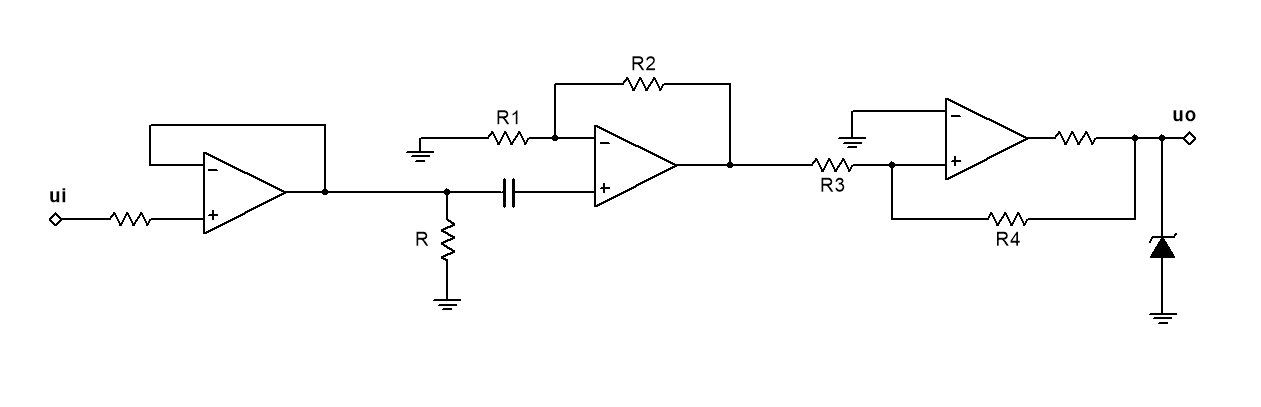
\includegraphics[scale=0.4]{fig/design/principle4.png}
            \caption{热释电测量电路第一版}
            \label{fig:design_prin_4}
        \end{figure}

        如图所示,输入信号首先经过一个跟随器以实现阻抗变换,增大输入内阻,
        然后输入信号通过一个一阶高通电路隔离直流分量,并适当放大变化电压幅值,
        最后通过滞回比较器来输出一个符合数字电压要求的电平。
        其中,如果输出由高电平变至低电平,则代表有人进入检测范围,如果由
        低电平变为高电平,则代表有人离开检测范围。

        但是这一版工作电路在我实际测量时发现主要存在以下几个问题:

        \begin{itemize}
            \item 所需要的电源种类过多。原因在于电路中的运放在第一版设计中,需要正负12V供电。
            但是由于我的电路最初为12V直流电池供电,所以并不能直接提供这两种电平。
            这导致电路中需要具备相对比较复杂的正负电源电路才能解决问题。
            
            \item 电路出现误检测现象。
            有人缓慢离开检测范围时,热释电传感探头输出电压会出现幅值过小的问题。这时,如果仅仅是增大电压放大倍数,则会因为
            有效信号和环境噪声幅值相近,输出电压会多次翻转,最终电平的高低与人是否离开检测范围没有确定关系。

        \end{itemize}

        为了解决上述问题,我设计的第二版热释电传感电路如图\ref{fig:design_prin_5}所示。

        \begin{figure}[H]
            \centering
            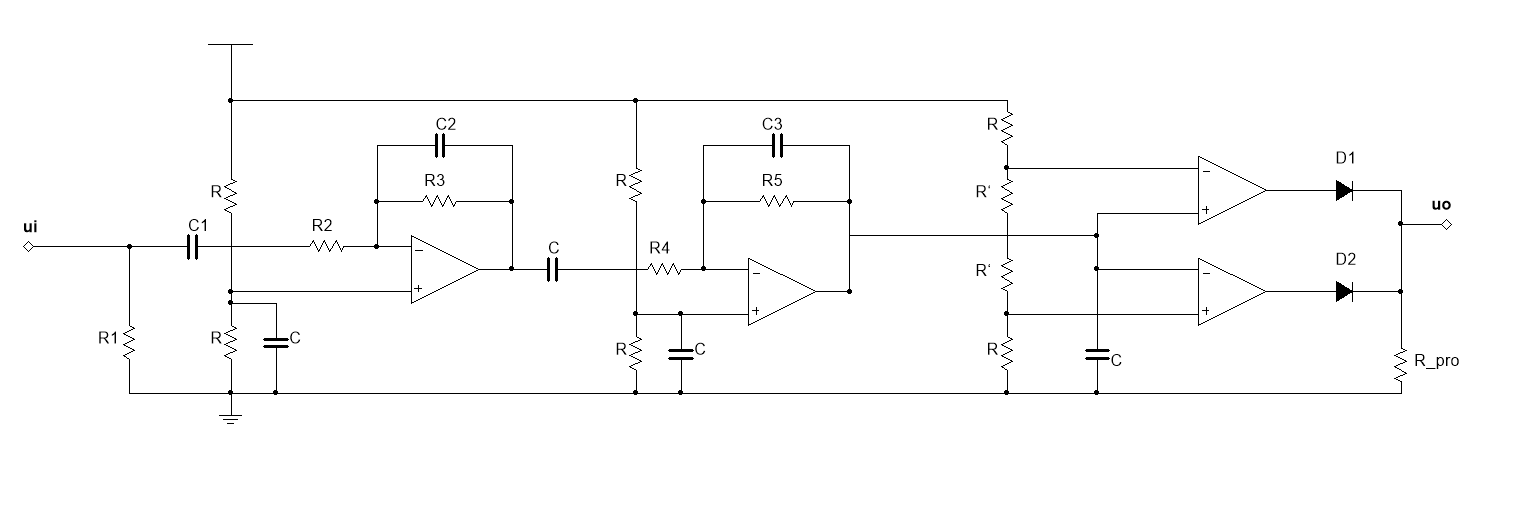
\includegraphics[scale=0.4]{fig/design/principle5.png}
            \caption{热释电传感电路第二版}
            \label{fig:design_prin_5}
        \end{figure}

        其中,R1和C1构成第一级高通滤波器,负责过滤直流电平,
        然后输入信号经过第一级高通滤波电路进一步滤波,并通过R2,R3
        实现电压放大。
        之后输入信号通过C进一步隔离直流风量,并通过第二级电路进行输出值幅值调整并进一步滤波。
        随后,输入信号通过一个双限电压比较器进行电压比较,在有人进出电路能输出一个高电平。

        针对第一版电路中存在的问题,我做了如下几点改进:
        \begin{itemize}
            \item 针对第一个问题,第二版电路中的运放都用5V 和 0V 供电。
            并且将电路中各个基准电位用R和C控制为2.5v。这样
            电路中就仅仅需要0V和5V的电源供电。
            
            \item 针对第二个问题,我将最后一级滞回比较器改为一个窗口比较器。这样做可以让电路在无人进出时输出一个
            低电平,只有在有人进出检测范围时输出一个高电平。虽然此时,仍然存在人缓慢离开而导致的电路误触现象,但是此时
            可以通过在后一级 MCU 内增加一个最小缓冲时间(即认为在输出电压变化后一定时间内,电压的再次变化为环境噪声所致,
            可以忽略)来抑制环境噪声。

            这样做的缺点在于,电路输出值电平高低与是否有人在检测范围内并没有明确的逻辑对应关系,而仅仅能判断
            是否有人进出检测范围。但这样的改进结果已经优于第一版电路中,输出电平的高低和是否检测到人之间逻辑
            对应关系可能因环境噪声而错误的结果。

        \end{itemize}

        窗口比较器的输入电压为:

        \begin{equation}
            u_{in} = \frac{R_5}{R_4} \frac{R_3}{R_2} \Delta u_i
        \end{equation}

        其中,$\frac{R_5}{R_4}$ 负责进行交流信号的放大部分,而
        $\frac{R_3}{R_2}$ 负责调整(放大或者减小)输入窗口比较器的输入电压以满足
        窗口比较器的电压比较要求。

        窗口比较器的两个阈值输入电压为:
        \begin{equation}
            \begin{cases}
                u_{l} = \frac{R}{2(R + R')} \\
                u_{h} = \frac{R+2R'}{2(R + R')} 
            \end{cases}
        \end{equation}


        \item 升压斩波电路

        在我们学习过的电路中,并没有一种模拟电路能实现DC/DC升压的效果。在经过调查后,我发现,
        通常使用的升压电路为升压斩波电路(BOOST)。由于身边没有合适的电感,所以对于这一部分电路我
        选择直接购买现有的模块,而不是自己从头搭建。所以,尽管其作为模拟电路,其详细原理在此并不详细叙述,
        仅仅假设其不仅能够有效升压,还拥有足够的功率输出能力。

    \end{enumerate}

    \subsection{数字电路模块}

    \begin{enumerate}
        \item 18650 12V直流电源

        电路的电源来源于18650 12V锂电池。
        其电池容量为2600mAH,瞬时最大输出功率为60W,经过大致估算,从输出功率和电池容量上来说,
        应该是满足我的项目需要的。
        
        \item 12V DC 风扇
        
        %figure 2 

        我购买的为AFB0812M 12V直流风扇。当供电电平为12V时,其最大所需电流(根据规格说明)大致在0.18A左右。
        由于风扇存在机械转动,所以风扇应该为电路功率消耗的最主要的来源。经过估算,在使用18650锂电池的情况下,
        风扇大致可转动14小时,所以从功率消耗上是满足要求的。

        \item L298N 电机驱动模块

        为了实现风扇转速可调,我使用了一个L298N 电机驱动模块来实现 pwm波控制风扇转速的功能。
        其原理是通过H桥电路,将主控板输出的幅值为5V的pwm波调制为幅值为12V的pwm波并输出给风扇,
        对于直流风扇而言,在输入的pwm波占空比不同时,相当于在风扇两端加不同电平的直流电压,
        从而实现风扇转速可调的功能。

        \item Arduino Mega 控制板

        我使用的主控板为Arduino Mega2560,其外设包括:
        \begin{itemize}
            \item 数字量输入输出口,其电平变化范围为0-5V
            \item 模拟量输入口,电平检测范围为0-5V
            \item pwm 输出口,可以输出幅值为0-5V,占空比不同的 pwm 波
            \item 中断输入口,可以用于检测热释电传感器输出值变化
            \item 5个串行输入输出口,可以用于实现蓝牙调试和连接
            \item IIC总线,可以用于与LCD显示屏之间的数据通信
        \end{itemize}

        Arduino Mega 上的外设是满足我的项目需求的。

        \item LCD显示屏

        我使用的显示屏为LCD1602 显示屏。其使用方式比较简单。它通过IIC总线和主控板之间进行数据传输。
        主控板通过IIC总线来写入LCD1602上一块RAM内存,然后由显示屏根据其上RAM的内容来显示对应信息。 
      
        在本项目中,我使用LCD显示屏来实现来显示实时温度测量结果和是否有人进出热释电传感器检测范围的判断结果。

        \item 蓝牙模块

        蓝牙模块原理十分简单,其基本原理基于串口通信,在进行波特率设置和通信协议设置后,可以将其直接视为普通串口通信来
        使用。

        而对应的APP可以使用上个暑季小学期所掌握的QT5开发框架来实现移动端的程序编写。

    \end{enumerate}

\section{模拟电路仿真结果}

    \subsection{5V稳压电路}

    仿真电路如图\ref{fig:sim1}所示:
    \begin{figure}[H]
        \centering
        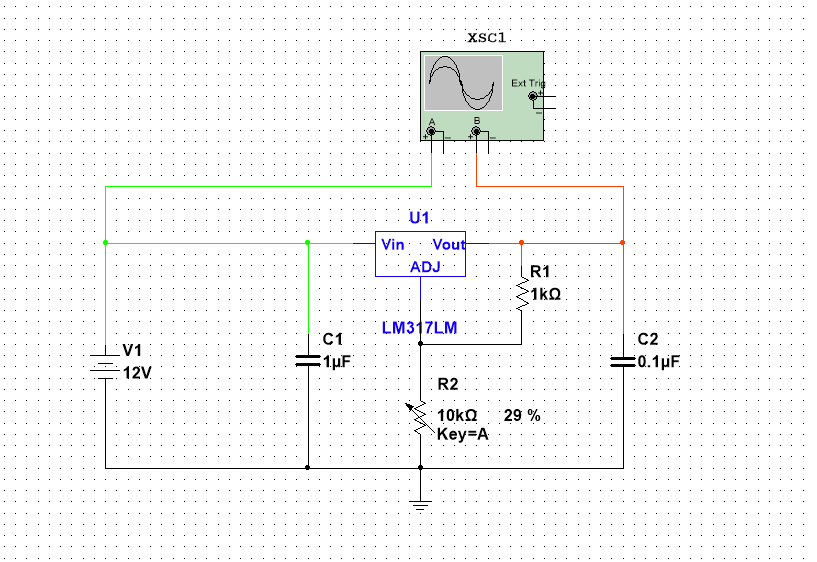
\includegraphics[scale=0.4]{fig/sim/sim1.png}
        \caption{5V稳压仿真电路}
        \label{fig:sim1}
    \end{figure}
    
    这里我使用了一个$10 k \Omega $ 的滑动变阻器来调节电压关系。最终,在$R_2 = 2.9 k \Omega $ 
    时,电路的输出波形如图\ref{fig:sim1_result1}所示:

    \begin{figure}[H]
        \centering
        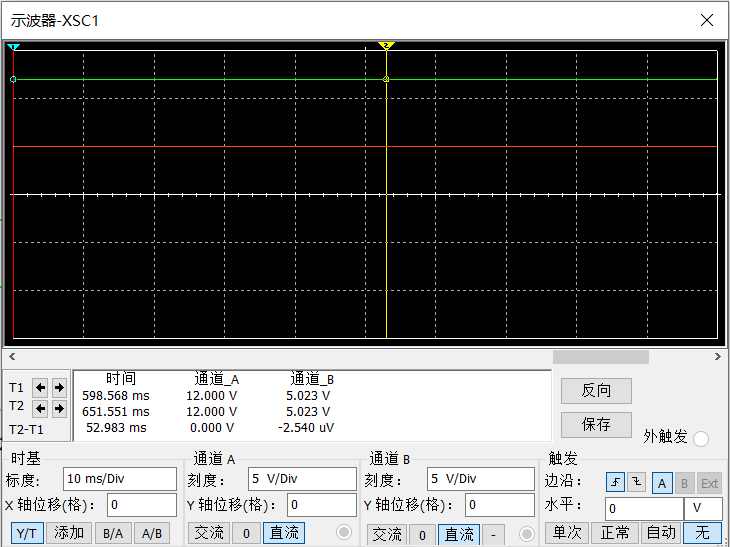
\includegraphics[scale=0.4]{fig/sim/sim1_result1.png}
        \caption{5V稳压电路输出波形}
        \label{fig:sim1_result1}
    \end{figure}
    可以看出,在输入电压基本不变时,输出电压比较稳定。

    该模块的传输特性曲线如图\ref{fig:sim1_result2}所示:
    \begin{figure}[H]
        \centering
        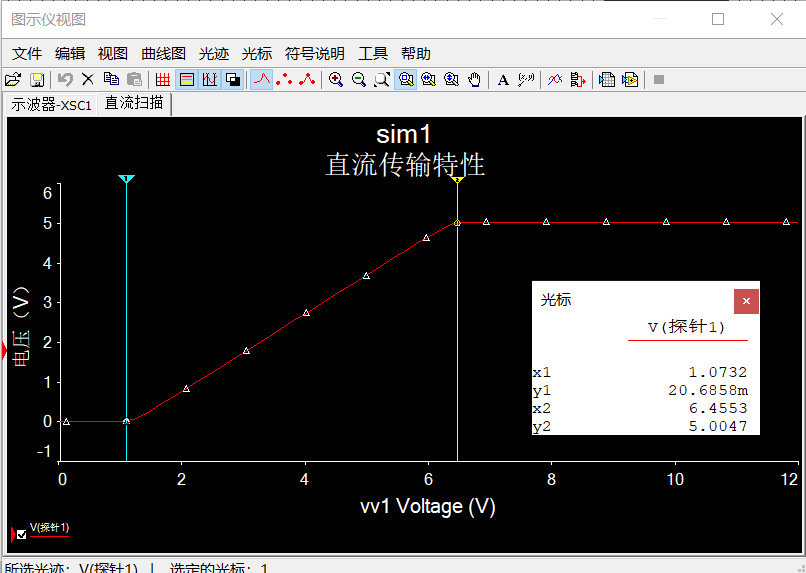
\includegraphics[scale=0.4]{fig/sim/sim1_result2.png}
        \caption{5V稳压仿真电路传输特性曲线}
        \label{fig:sim1_result2}
    \end{figure}
    
    从图中可见,只有当输入电压大于6.45V时,输出电压才能稳定在5V不变。

    在输入电压为12V时,电路的输出电压随后一级电路输入电阻的变化曲线如图\ref{fig:sim1_result3}所示。
    \begin{figure}[H]
        \centering
        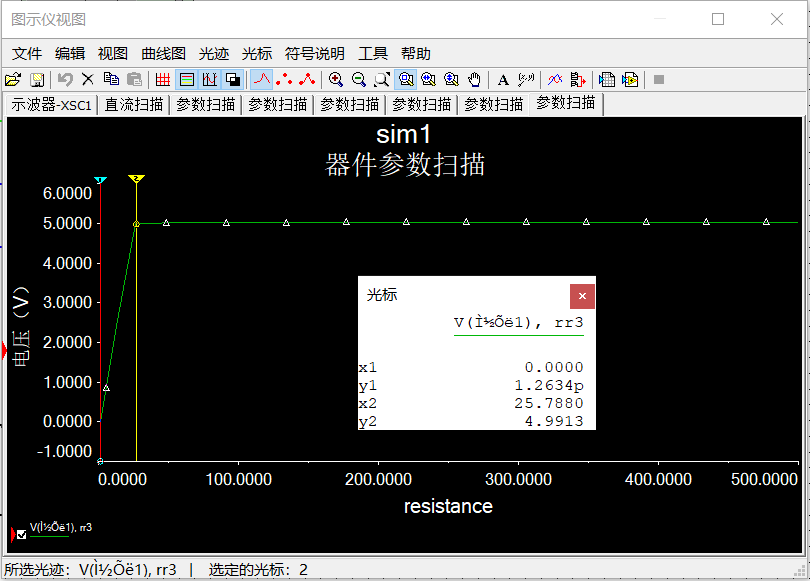
\includegraphics[scale=0.4]{fig/sim/sim1_result3.png}
        \caption{5V输出电压受后一级输入电阻的影响}
        \label{fig:sim1_result3}
    \end{figure}
    
    可以看出,只有当后一级电路的等效输入电阻大于$25 \Omega $ 时,输出电压才能稳定在5V。 
    电路带载能力较强。

    \subsection{正负电源电路}

    正负电源仿真电路如图\ref{fig:sim2}所示:
    \begin{figure}[H]
        \centering
        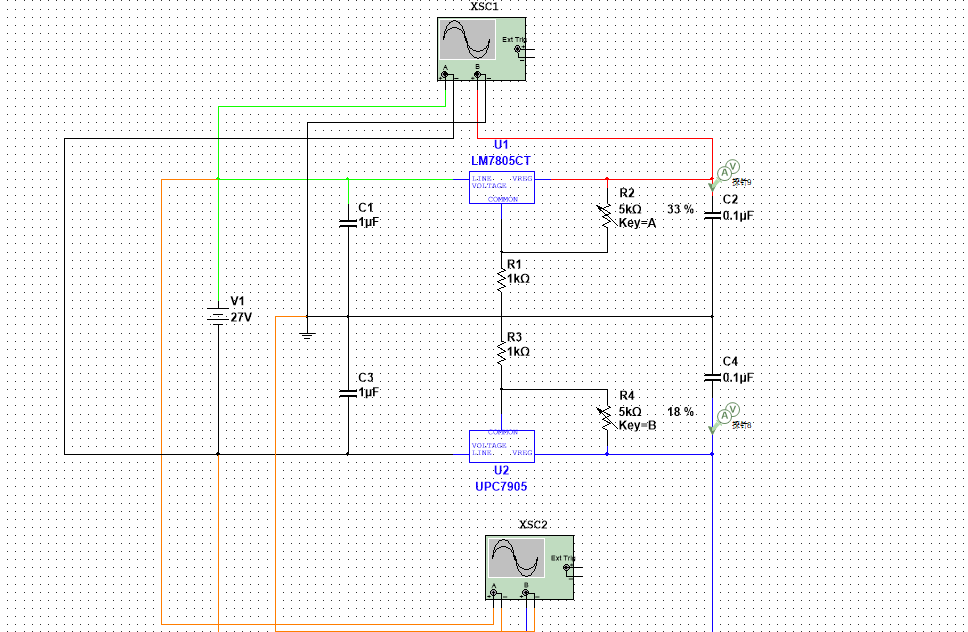
\includegraphics[scale=0.4]{fig/sim/sim2.png}
        \caption{正负电源电路}
        \label{fig:sim2}
    \end{figure}

    当$R_2 = 1.65 k\Omega , R_4 = 0.9k \Omega$时,电路的正负电源输出如图\ref{fig:sim2_result1},\ref{fig:sim2_result2}所示:

    \begin{figure}[H]
        \centering
        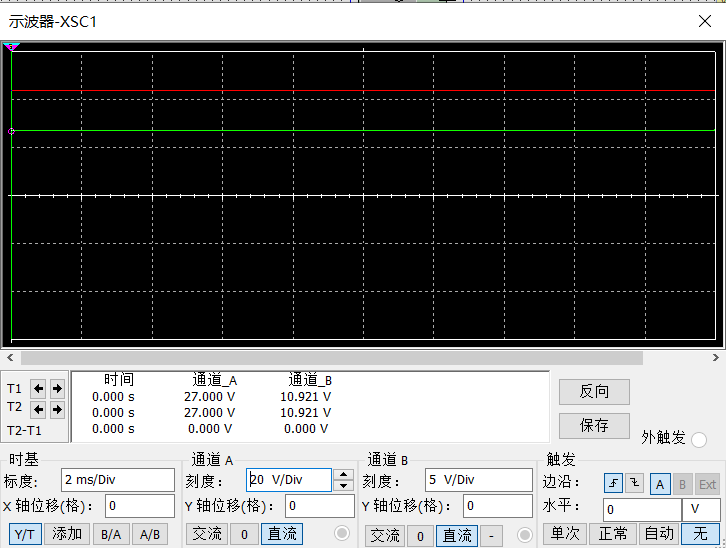
\includegraphics[scale=0.4]{fig/sim/sim2_result1.png}
        \caption{正电源输出波形}
        \label{fig:sim2_result1}
    \end{figure}
    
    \begin{figure}[H]
        \centering
        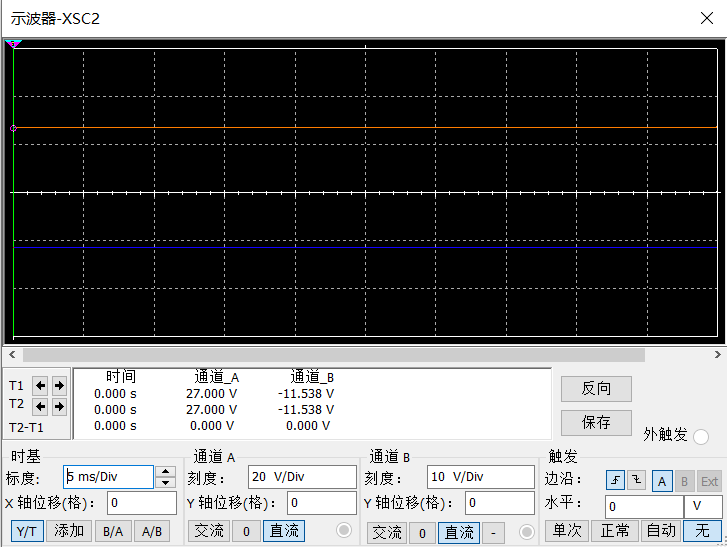
\includegraphics[scale=0.4]{fig/sim/sim2_result2.png}
        \caption{负电源输出波形}
        \label{fig:sim2_result2}
    \end{figure}
    
    此时,正电源$ V_+ \approx 10.9V$,负电源$V_- \approx -11.6 V$。已经满足了后续运放的电压放大需求。
    
    此时,电路的传输特性曲线如图\ref{fig:sim2_result3}所示:

    \begin{figure}[H]
        \centering
        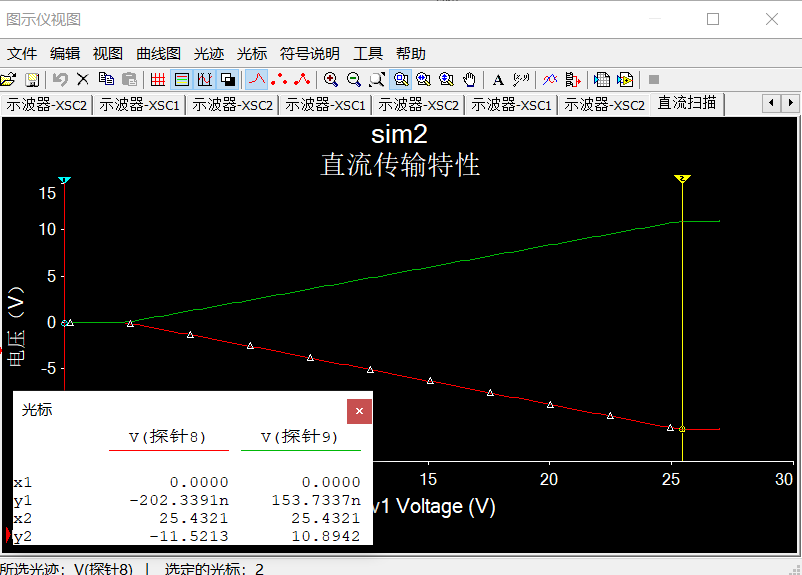
\includegraphics[scale=0.4]{fig/sim/sim2_result3.png}
        \caption{电路传输特性曲线}
        \label{fig:sim2_result3}
    \end{figure}
    
    从传输特性曲线中可以看出,要想让电路正常工作,需要保证前一级电路,即升压斩波电路输出电压大于25V。

    而后一级电路的等效输入电阻对于输出电压的影响曲线如图\ref{fig:sim2_result4},\ref{fig:sim2_result5}所示:
    \begin{figure}[H]
        \centering
        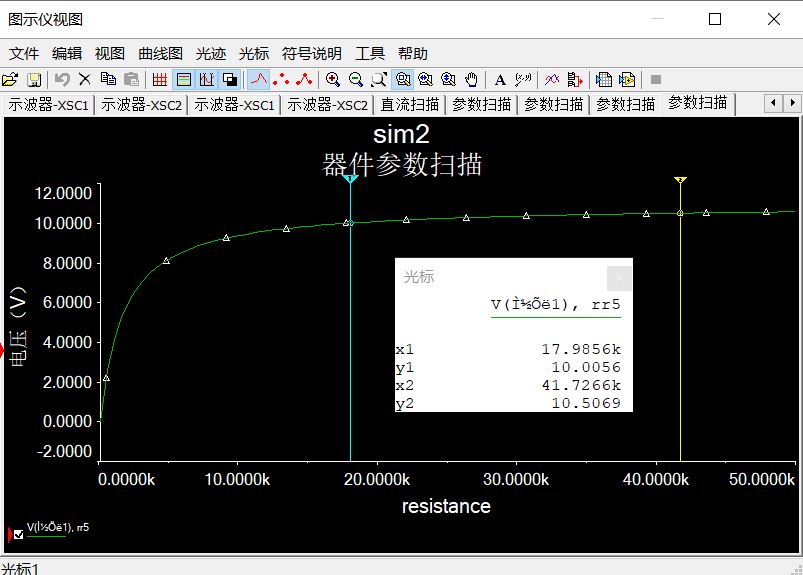
\includegraphics[scale=0.4]{fig/sim/sim2_result4.png}
        \caption{后一级电路输入电阻对于正电源影响}
        \label{fig:sim2_result4}
    \end{figure}
    
    \begin{figure}[H]
        \centering
        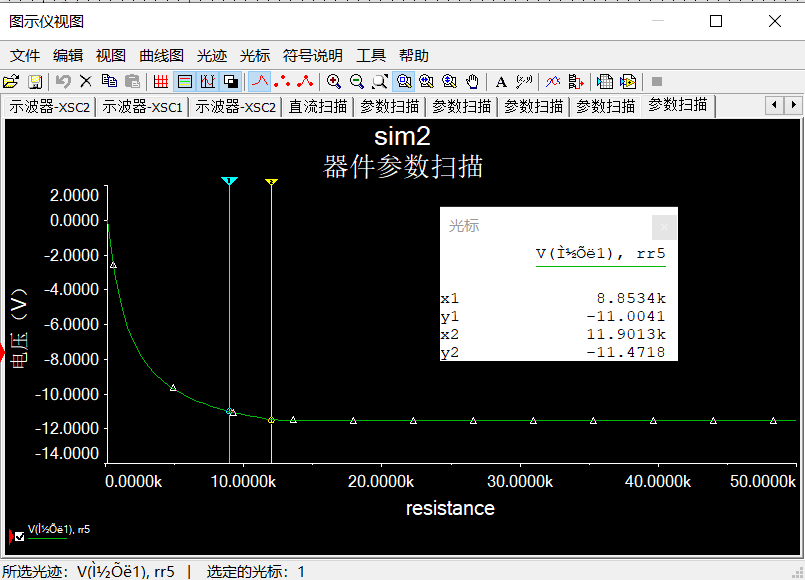
\includegraphics[scale=0.4]{fig/sim/sim2_result5.png}
        \caption{后一级电路输入电阻对于负电源影响}
        \label{fig:sim2_result5}
    \end{figure}
    
    可以看出,为获得期望的输出电压,正电源需要保证后一级电路输入电阻大于$41k\Omega$ ,负电源需要保证输入电阻大于$11.9k\Omega$。
    这说明电路带载能力较差。在实际搭建过程中,可以考虑用由功放构成的跟随器作为缓冲级电路以增强电路带载能力。

    \subsection{温度测量电路}

    温度测量电路的仿真电路如图\ref{fig:sim3}所示:
    \begin{figure}[H]
        \centering
        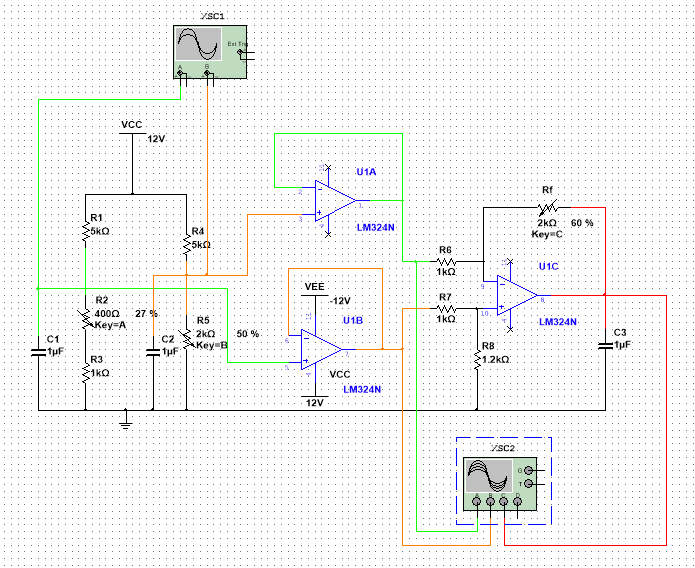
\includegraphics[scale=0.4]{fig/sim/sim3.png}
        \caption{温度测量仿真电路}
        \label{fig:sim3}
    \end{figure}
    
    在这里,我使用了一个1k的电阻和一个可滑动的,阻值为400$\Omega$的电阻串联模拟铂电阻PT1000。每当该滑动变阻器阻值上升百分之一,
    就可以近似的看成环境温度上升1摄氏度。这意味着该滑动变阻器的百分比可以直接被近似看做环境温度。

    当$R_2$滑动变阻器的百分比为27\% (模拟环境温度27摄氏度),电桥两端的输出电压如图\ref{fig:sim3_result1}所示:
    \begin{figure}[H]
        \centering
        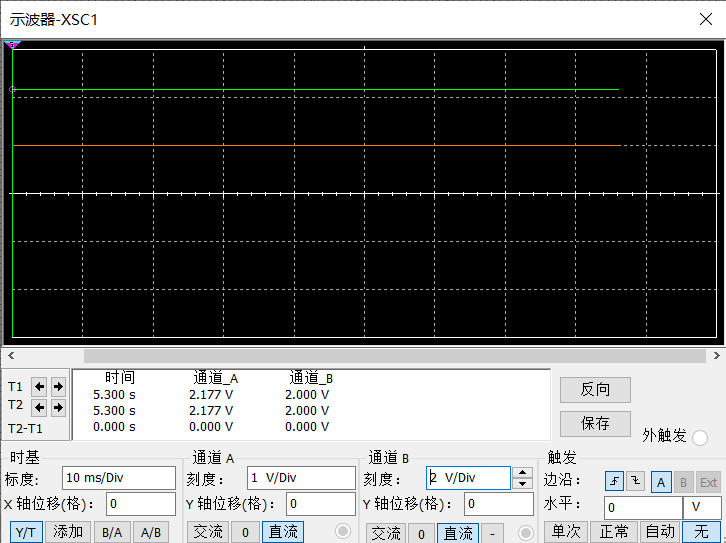
\includegraphics[scale=0.4]{fig/sim/sim3_result1.png}
        \caption{电桥输出电压}
        \label{fig:sim3_result1}
    \end{figure}

    测量结果与近似计算式 (\ref{equ:approx}) 的计算结果基本一致。
    
    最终输出电压如图\ref{fig:sim3_result2}所示。

    \begin{figure}[H]
        \centering
        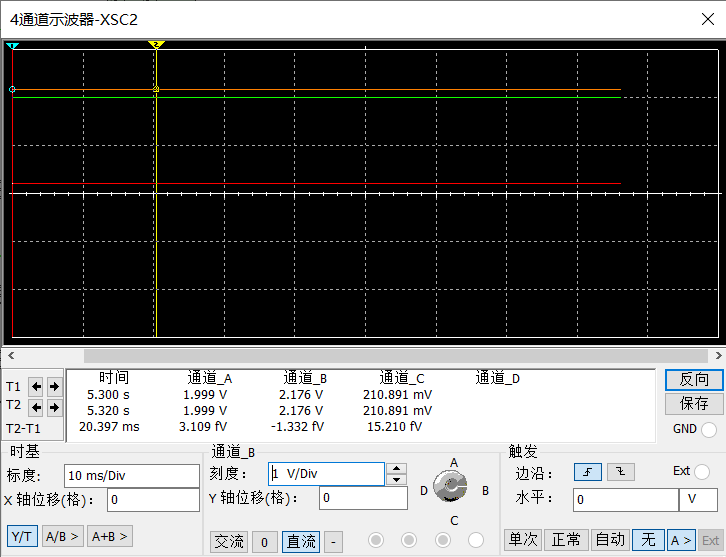
\includegraphics[scale=0.4]{fig/sim/sim3_result2.png}
        \caption{电路输出电压}
        \label{fig:sim3_result2}
    \end{figure}

    此时,在实际搭建电路,调整电路参数时,可以通过$\frac{R_f}{R_+}$来调节输出电压的变化范围,
    以满足主控板Arduino Mega 上 DAC芯片的电平转换范围。

    电路输出电压随温度($R_2$ 阻值)的变化特性如图\ref{fig:sim3_result3}所示:
    
    \begin{figure}[H]
        \centering
        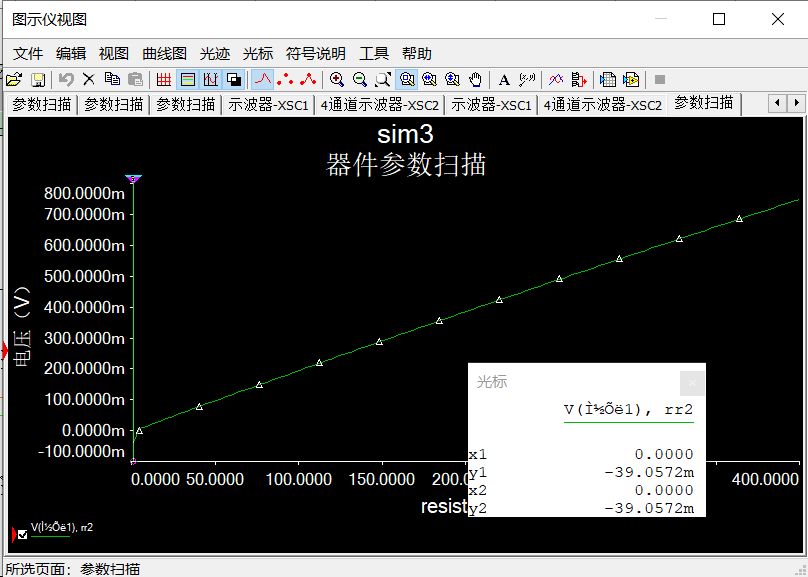
\includegraphics[scale=0.4]{fig/sim/sim3_result3.png}
        \caption{输出电压随温度变化的特性曲线}
        \label{fig:sim3_result3}
    \end{figure}
    
    可以看出,此时电路有足够好的线性性质,可以用于简单的温度测量。
    
    需要注意的是,在仿真中我使用的是LM324通用型运放,但是在实际搭接电路时,我使用的是OPA277精密运放来进一步提升电路精度。

    \subsection{热释电测量电路}

    由于我最终使用的,是我改版以后的第二版热释电测量电路,所以在这里只展示第二版电路的仿真结果。

    第二版热释电测量电路的仿真电路如图\ref{fig:sim4}所示:

    \begin{figure}[H]
        \centering
        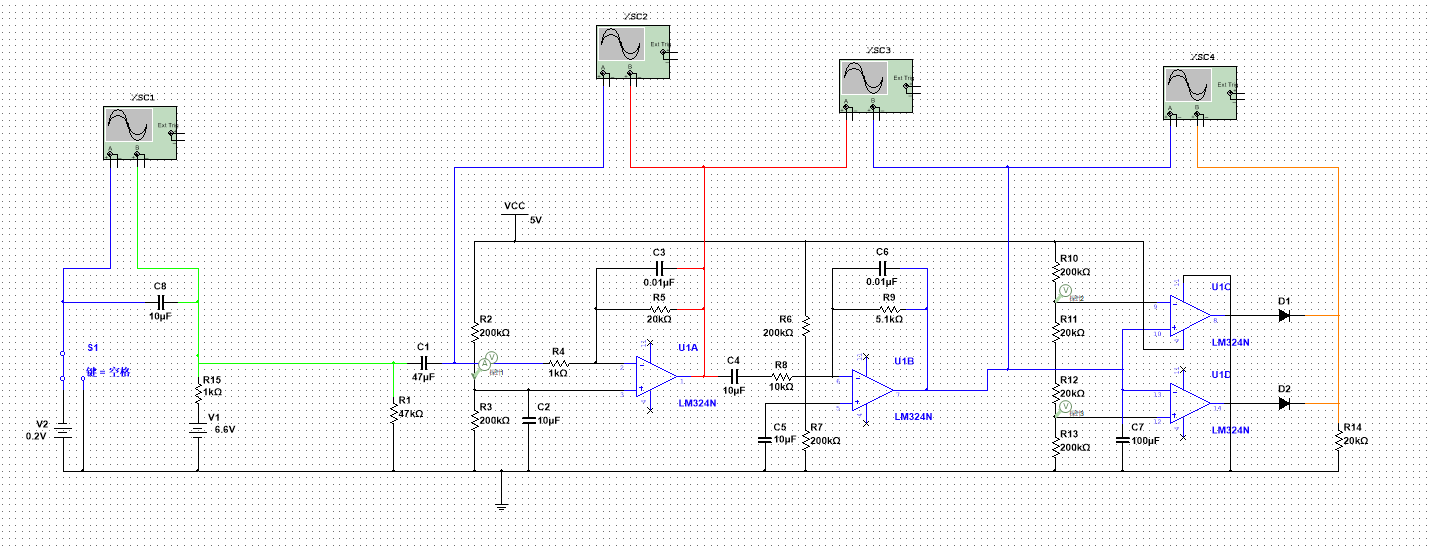
\includegraphics[scale=0.4]{fig/sim/sim4.png}
        \caption{热释电测量仿真电路}
        \label{fig:sim4}
    \end{figure}
    
    在仿真时,我使用了一个RC电路加一个单刀双掷开关来模拟传感器的输入电压变化过程。在无人进出检测范围时,输入电平基本维持在一个
    直流电压稳定不改变。当有人进入检测范围时,电平先有大约200mV的压降,然后逐渐恢复至原电压水平;当有人离开检测范围时,
    电平先有大约200mV的压升,然后逐渐恢复为原电压水平。

    (模拟)传感器输入波形如图\ref{fig:sim4_result2},\ref{fig:sim4_result3}所示:

    \begin{figure}[H]
        \centering
        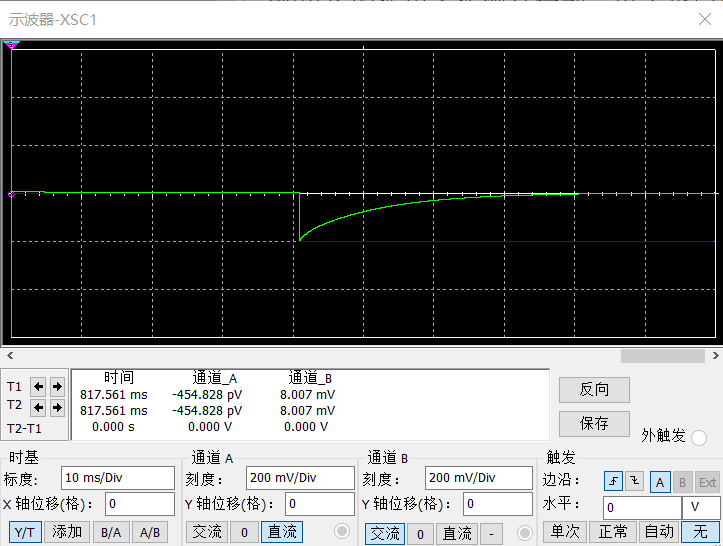
\includegraphics[scale=0.4]{fig/sim/sim4_result2.png}
        \caption{传感器输入波形-有人进入}
        \label{fig:sim4_result2}
    \end{figure}
    
    \begin{figure}[H]
        \centering
        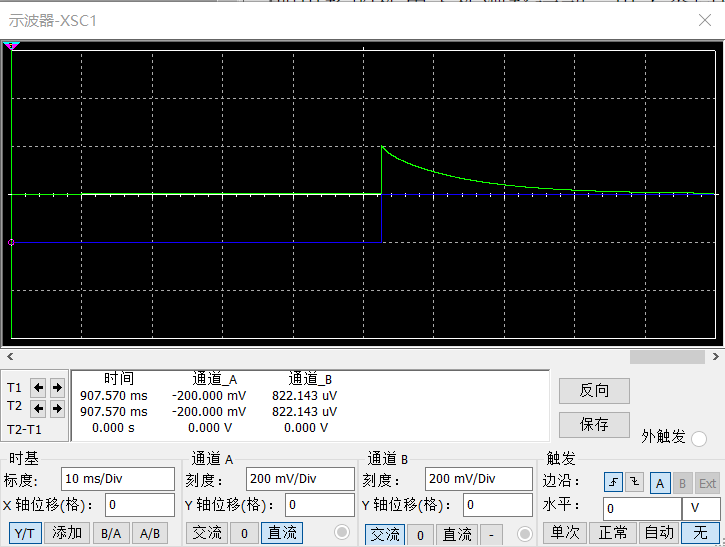
\includegraphics[scale=0.4]{fig/sim/sim4_result3.png}
        \caption{传感器输入波形-有人离开}
        \label{fig:sim4_result3}
    \end{figure}

    在两种不同的情况下,第一级电路的输出波形分别如图\ref{fig:sim4_result5},\ref{fig:sim4_result4}所示:

    \begin{figure}[H]
        \centering
        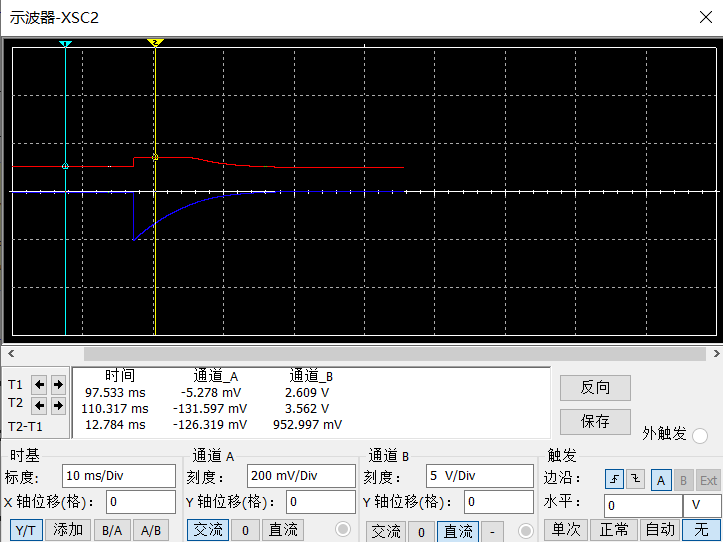
\includegraphics[scale=0.4]{fig/sim/sim4_result5.png}
        \caption{第一级输出波形-有人进入}
        \label{fig:sim4_result5}
    \end{figure}

    \begin{figure}[H]
        \centering
        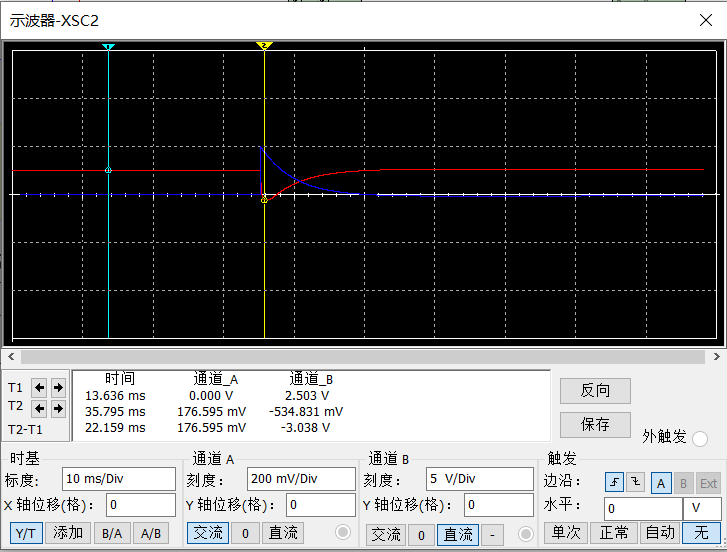
\includegraphics[scale=0.4]{fig/sim/sim4_result4.png}
        \caption{第一级输出波形-有人离开}
        \label{fig:sim4_result4}
    \end{figure}

    可以看出,此时第一级电路输出的最高电平为3.5V,输出的最低电平为-0.5V。可以被第二级电路有效识别。

    此时第二级电路输出波形如图\ref{fig:sim4_result9},\ref{fig:sim4_result8}所示:

    \begin{figure}[H]
        \centering
        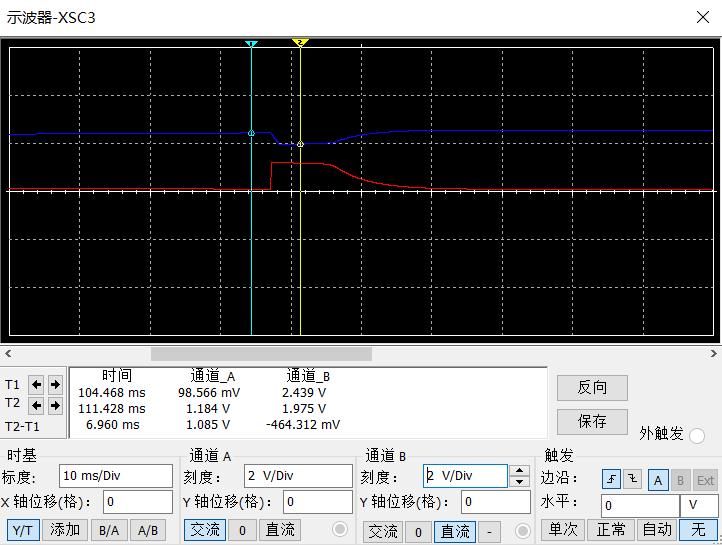
\includegraphics[scale=0.4]{fig/sim/sim4_result9.png}
        \caption{第二级输出波形-有人进入}
        \label{fig:sim4_result9}
    \end{figure}

    \begin{figure}[H]
        \centering
        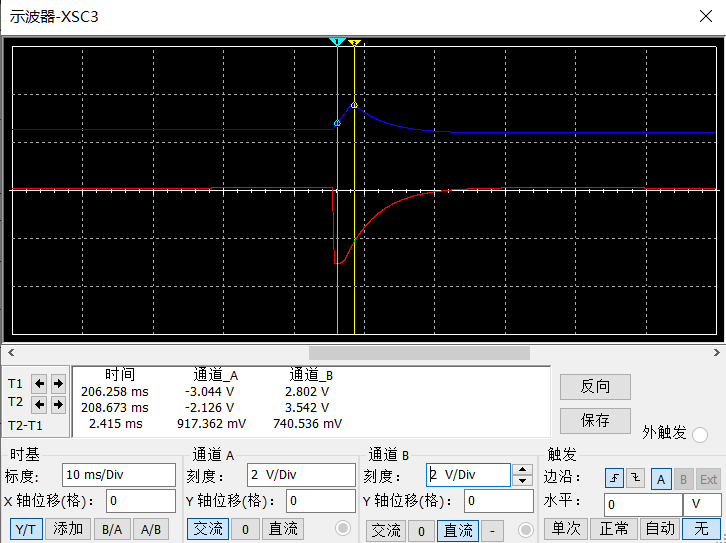
\includegraphics[scale=0.4]{fig/sim/sim4_result8.png}
        \caption{第二级输出波形-有人离开}
        \label{fig:sim4_result8}
    \end{figure}

    
    此时,第二级电路经过一定比例的电平缩小以后,其输出的最高电平为3.5V,输出的最低电平为1.98V。可以被后一级窗口比较器识别。

    最后一级电路的输出波形如图\ref{fig:sim4_result11},\ref{fig:sim4_result10}所示:
  
    \begin{figure}[H]
        \centering
        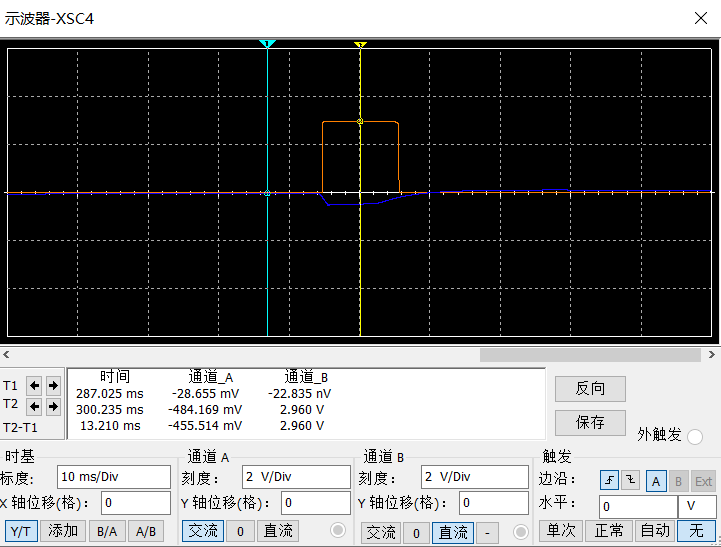
\includegraphics[scale=0.4]{fig/sim/sim4_result11.png}
        \caption{最终输出波形-有人进入}
        \label{fig:sim4_result11}
    \end{figure}
    
        \begin{figure}[H]
        \centering
        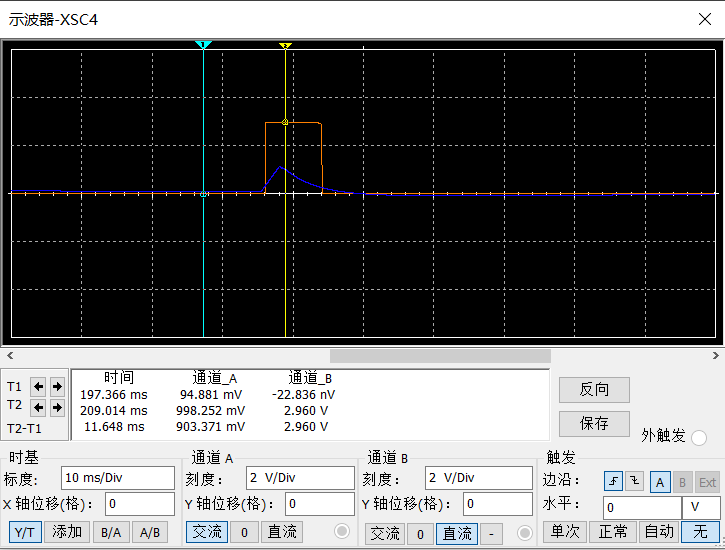
\includegraphics[scale=0.4]{fig/sim/sim4_result10.png}
        \caption{最终输出波形-有人离开}
        \label{fig:sim4_result10}
    \end{figure}

    可以看出,在有人进出检测范围时,最后一级电路都可以正常输出一个矩形波。

    对于电路的响应恢复速度,测量结果如图\ref{fig:sim4_result7},\ref{fig:sim4_result6}所示:

    \begin{figure}[H]
        \centering
        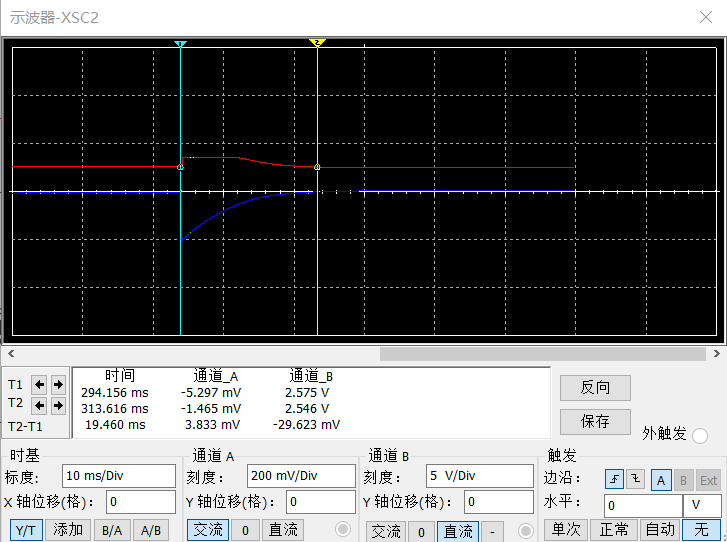
\includegraphics[scale=0.4]{fig/sim/sim4_result7.png}
        \caption{电路响应时间-下降}
        \label{fig:sim4_result7}
    \end{figure}
    
    \begin{figure}[H]
        \centering
        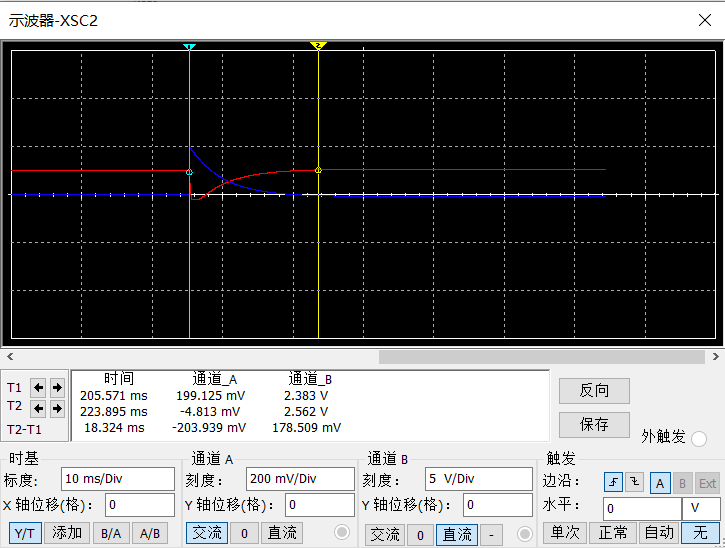
\includegraphics[scale=0.4]{fig/sim/sim4_result6.png}
        \caption{电路响应时间-上升}
        \label{fig:sim4_result6}
    \end{figure}
    
    可见,不论是人进入检测范围还是人离开检测范围,系统的响应恢复时间都在20mS以内。
    这说明在现实世界中,电路是可以及时为下一次人的动作变化做好准备的。

    至此,所有由自己搭建的模拟电路模块仿真完成。

\section{电路搭建与实测结果}

    \subsection{模拟电路模块}
\begin{enumerate}
    \item 5V电源模块:
    
    我最终搭建的5V电源模块如图\ref{fig:module1}所示:
    \begin{figure}[H]
        \centering
        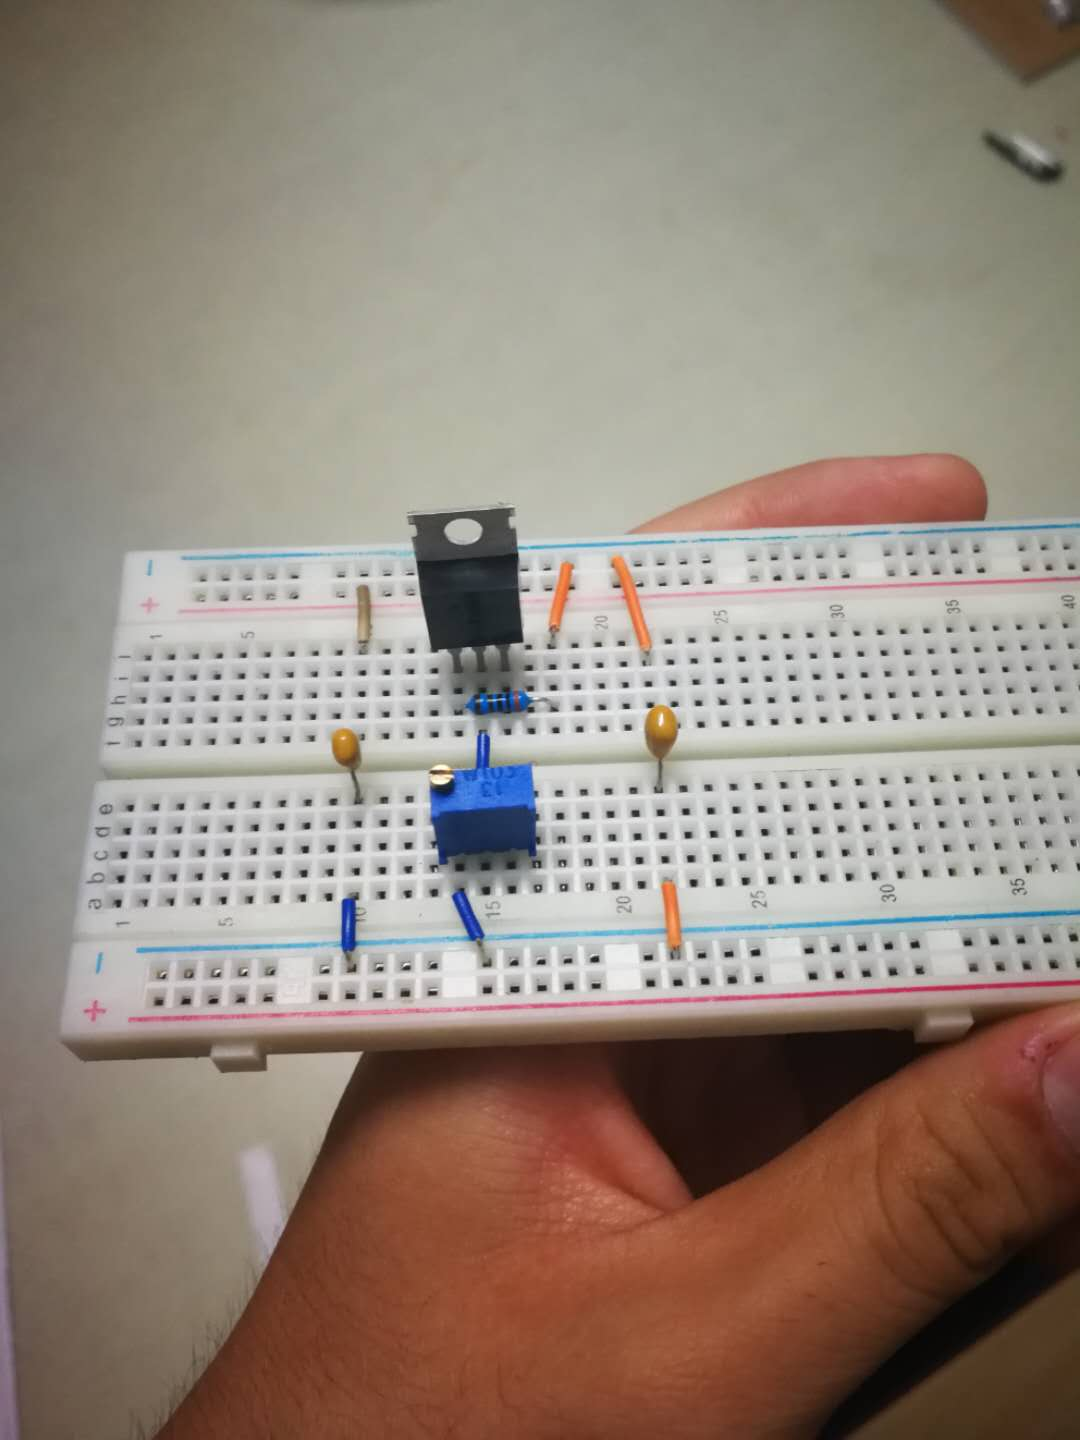
\includegraphics[scale=0.1]{fig/result/module1.png}
        \caption{5V电源模块}
        \label{fig:module1}
    \end{figure}
    
    经过调整,其最终的输出电平波形如图所示:

    \begin{figure}[H]
        \centering
        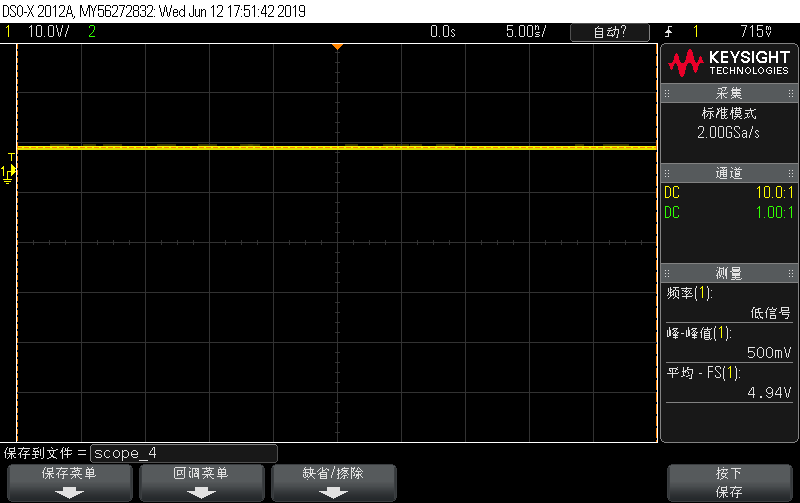
\includegraphics[scale=0.3]{fig/result/module1_result1.png}
        \caption{5V电源模块输出波形}
        \label{fig:module1_result1}
    \end{figure}
    
    最终输出电压为4.94V,近似为5V,已经满足下一级电路的电平需求,同时电压上下波动幅度大约只有0.1-0.2V,电路稳压性能较好。

    \item 正负电源模块
    
    我最终搭建的正负电源模块如图\ref{fig:module2}所示:
    \begin{figure}[H]
        \centering
        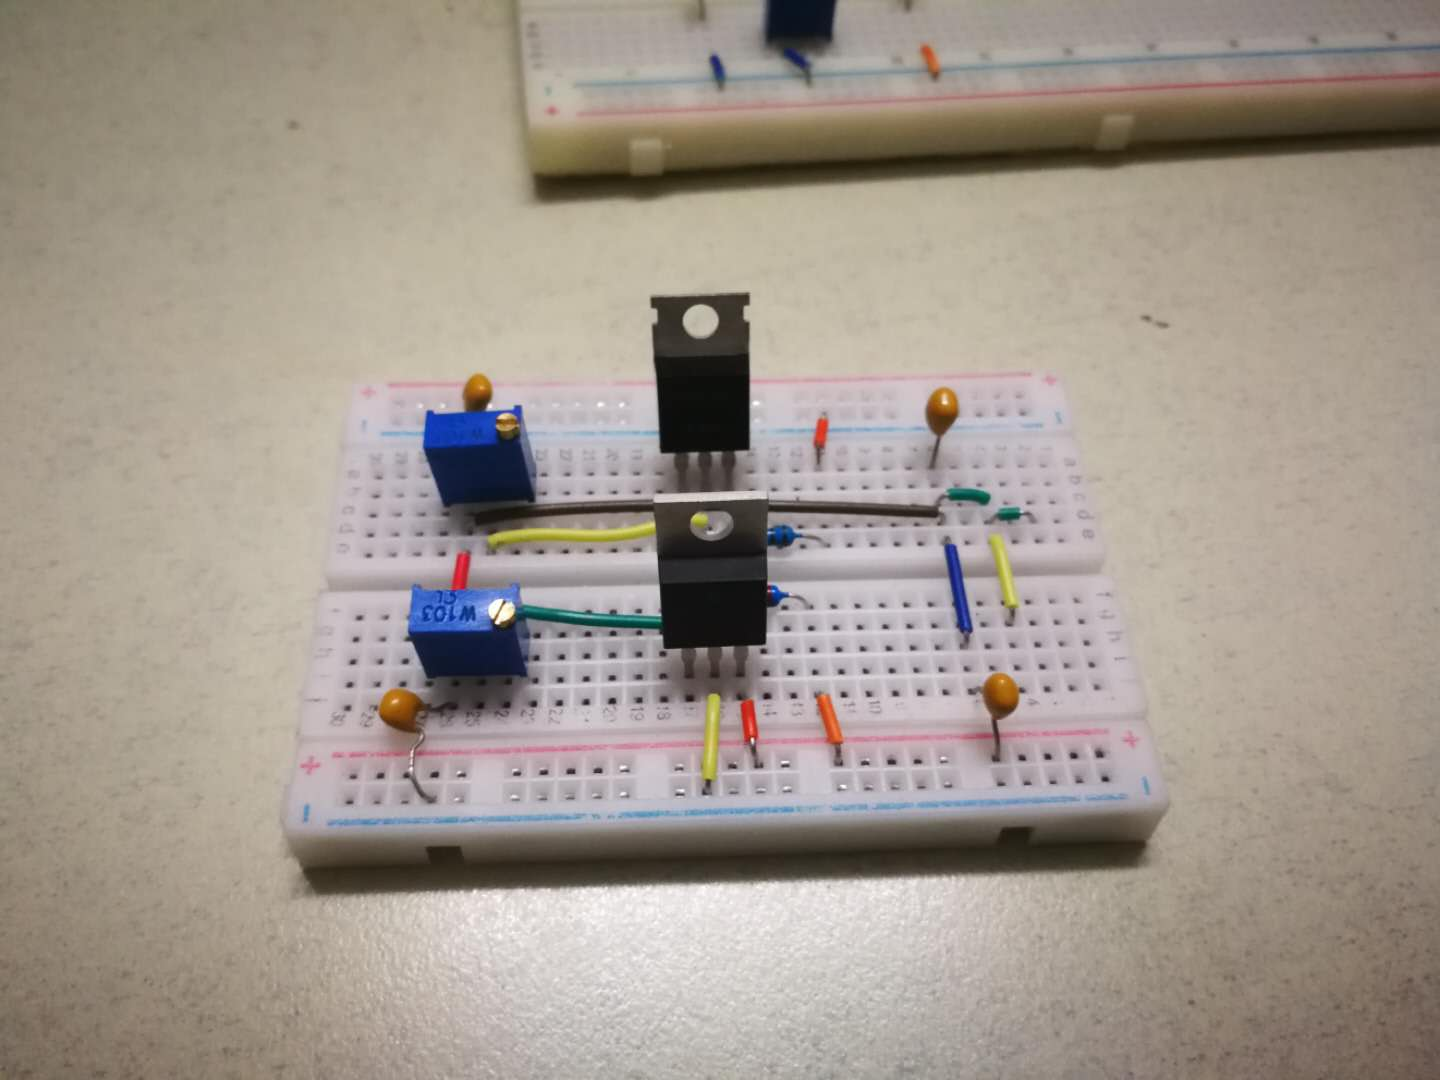
\includegraphics[scale=0.1]{fig/result/module2.png}
        \caption{正负电源模块}
        \label{fig:module2}
    \end{figure}

    在输入电压大于26V时,输出电压波形如图所示:
    \begin{figure}[H]
        \centering
        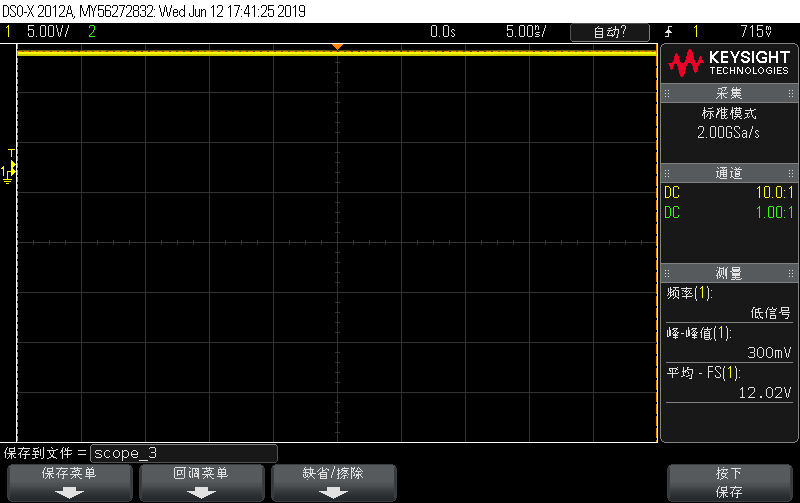
\includegraphics[scale=0.3]{fig/result/module2_result1.png}
        \caption{正电压输出波形}
        \label{fig:module2_result1}
    \end{figure}
    
    \begin{figure}[H]
        \centering
        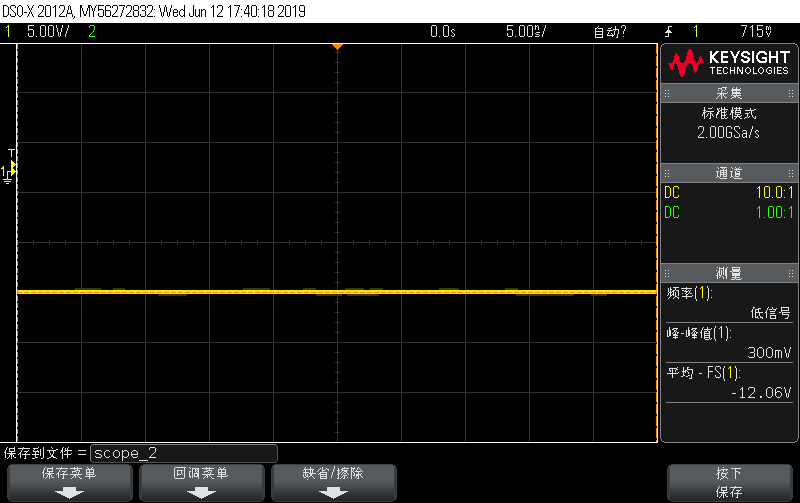
\includegraphics[scale=0.3]{fig/result/module2_result2.png}
        \caption{负电压输出波形}
        \label{fig:module2_result2}
    \end{figure}

    最终输出的正电压为12.02V,负电压为-12.06V,同时,电压稳定性能较好。但是如果直接在后一级加入电阻,则发现输出电平
    会降低,这说明电路的带载能力较弱。在引入功放构成的跟随器做缓冲级后,问题得到了解决。
    
    \item 温度测量模块
    
    我搭建的温度测量模块如图\ref{fig:module3}所示:
    \begin{figure}[H]
        \centering
        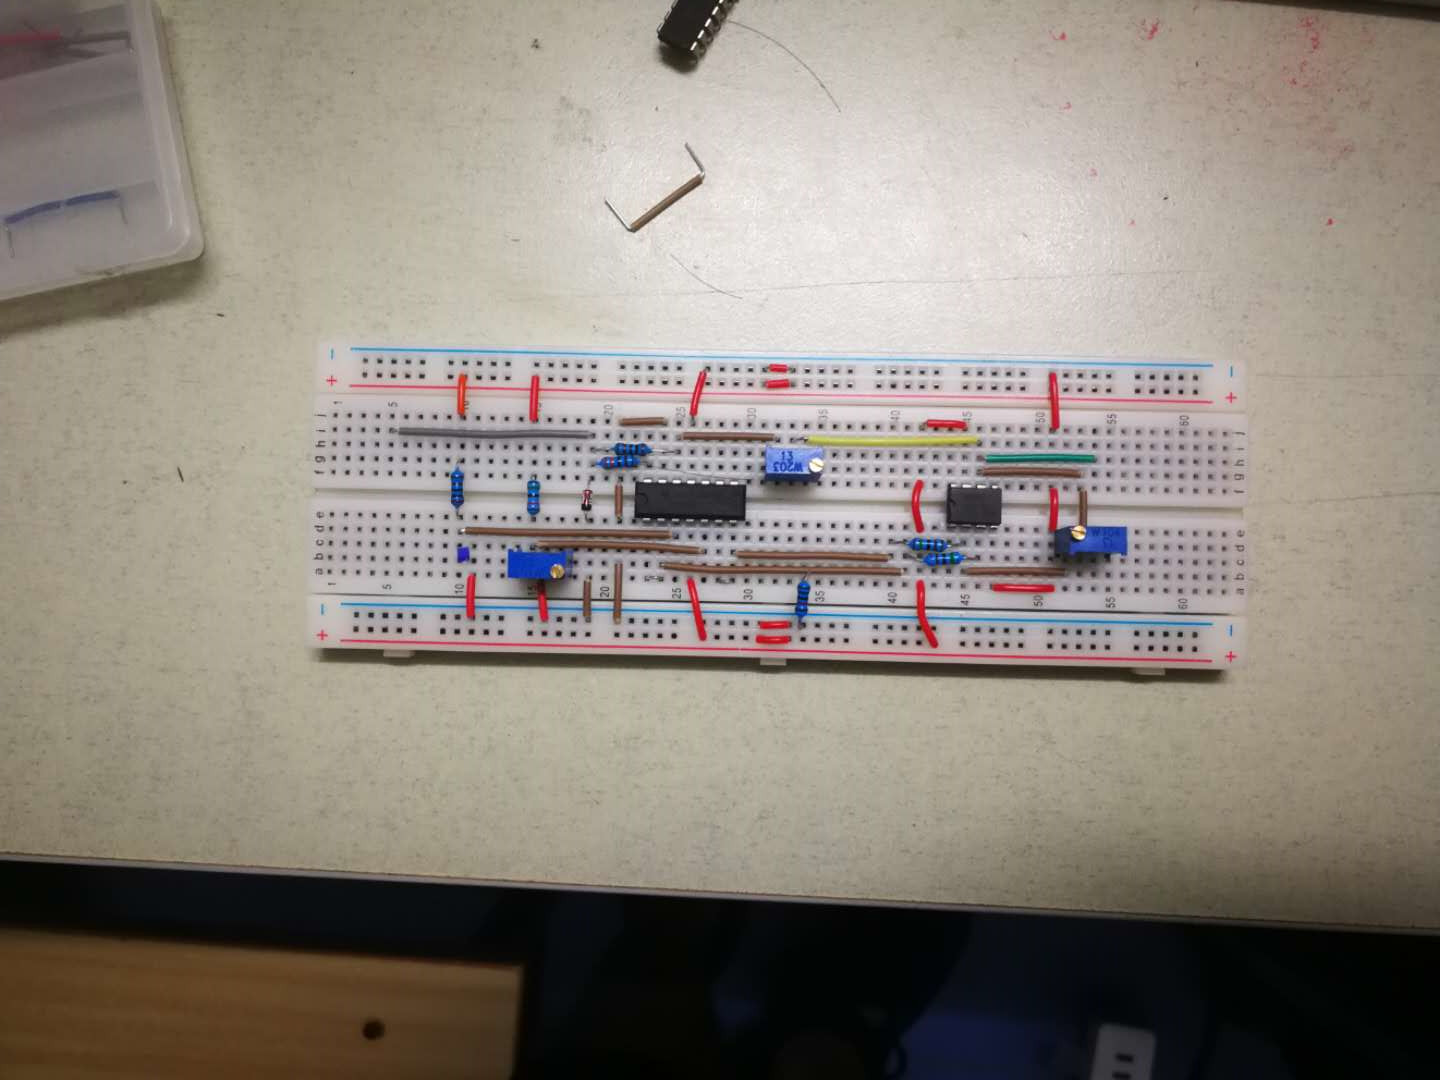
\includegraphics[scale=0.1]{fig/result/module3.png}
        \caption{温度测量模块}
        \label{fig:module3}
    \end{figure}
    
    其中,电压跟随器我仍然使用了LM324,但是运算电路部分使用了一个OPA277精密运放来提升电路运算精度。同时,我引入了多个可调变阻器
    来快速调节电路参数。

    最终,测得环境温度(用手持红外成像仪测量)和输出电压之间的关系如下表所示:

    \begin{table}[H]
        \centering
        \renewcommand\arraystretch{2}   %used to adjust space between lines 
        \begin{tabular}{cc}
        \toprule
            温度 $T / ^{\circ}C$ &  输出电压 $V_{out} / V$\\
        \midrule
             26 & 0.261 \\ 
             29 & 0.279 \\ 
             31 & 0.299 \\ 
        \bottomrule
        \end{tabular}
        \caption{温度和输出电压之间的关系}
        \label{tab:module3_result}
    \end{table}
    
    由于测试条件所限,只能测得这3组比较有代表性的输入。根据验算可知,这三点基本在一条直线上,由于数据量较少,
    所以在此并不做数据拟合。

    对于Arduino Mega主控板的ADC芯片,通过调整前一级电压放大倍数,
    环境温度可以通过公式\ref{equ:temprature}近似计算:

    \begin{equation}
        temp = (read_in) / 2 \label{equ:temprature} 
    \end{equation}

    其中,read\_in为ADC芯片所读取值(变化范围为0-1023)。虽然这样一来温度测量精度只有0.5摄氏度,
    但是对于相对简单的风扇调节应用来说已经满足其基本需求。

    \item 热释电传感模块

    我搭建的热释电传感模块如图\ref{fig:module4_1},\ref{fig:module4_2}所示:

    \begin{figure}[H]
        \centering
        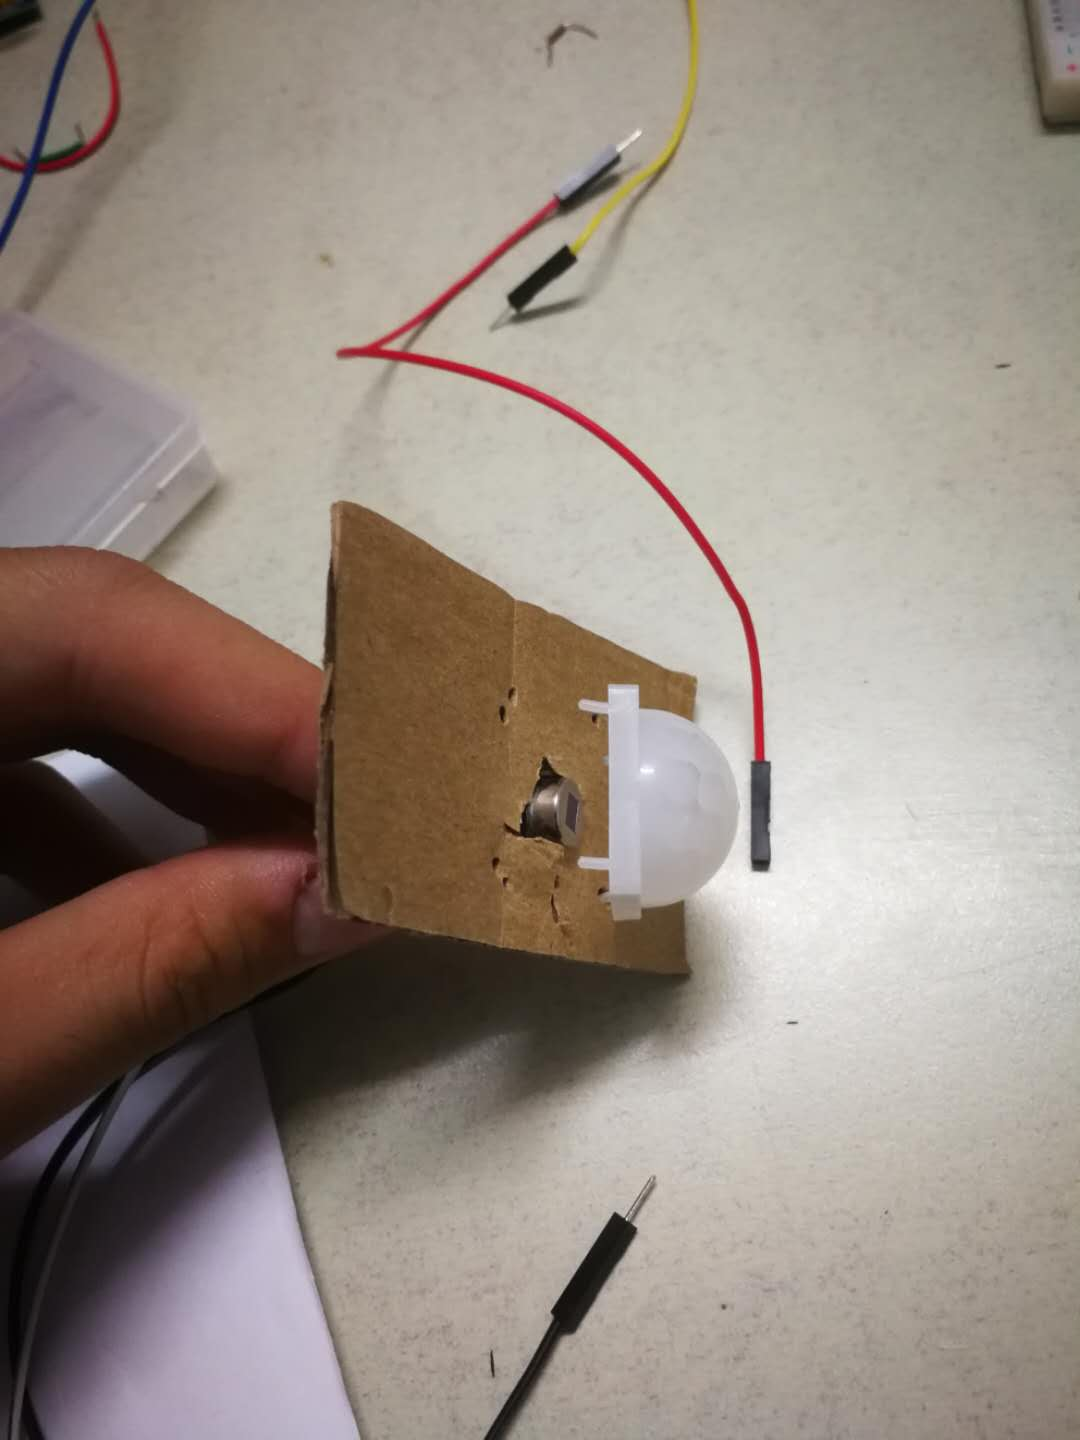
\includegraphics[scale=0.1]{fig/result/module4_1.png}
        \caption{自制热释电传感探头}
        \label{fig:module4_1}
    \end{figure}
    
    \begin{figure}[H]
        \centering
        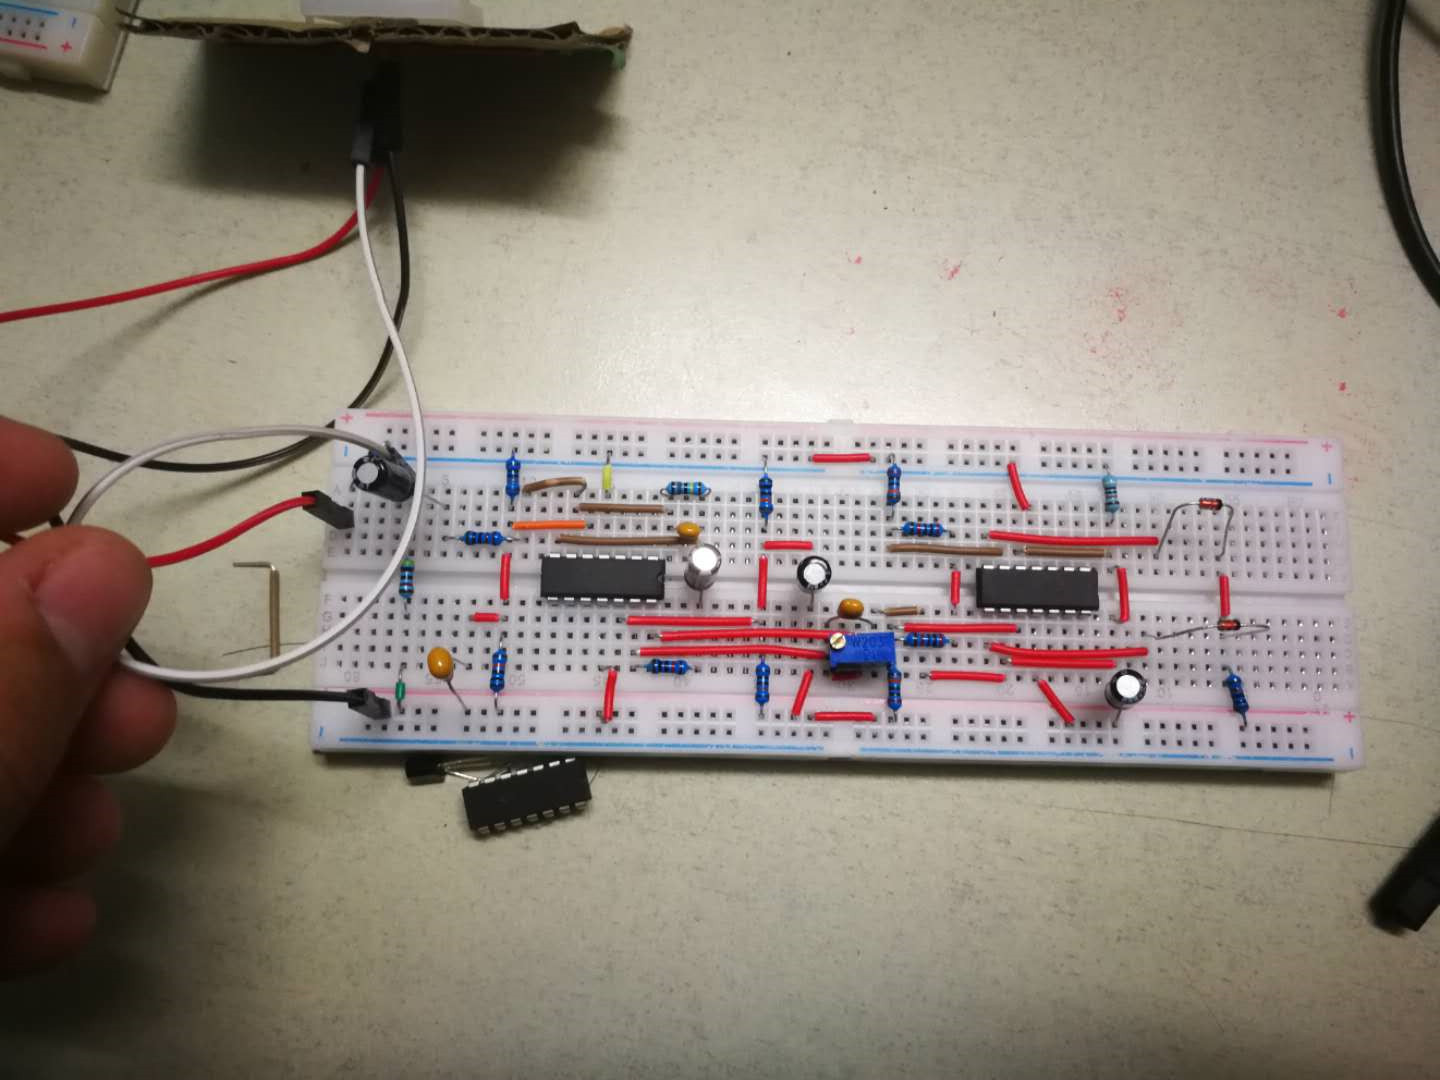
\includegraphics[scale=0.1]{fig/result/module4_2.png}
        \caption{热释电传感实验电路}
        \label{fig:module4_2}
    \end{figure}
    
    其中,图\ref{fig:module4_1}为我自己用硬纸板和绝缘胶带制作的带有菲涅尔滤镜的热释电探头,图\ref{fig:module4_2}为我搭建的
    热释电实验电路。

    最终,在有人进出检测范围(实际测量大约为20cm)时,电路输出波形如图\ref{fig:module4_result1}所示:

    \begin{figure}[H]
        \centering
        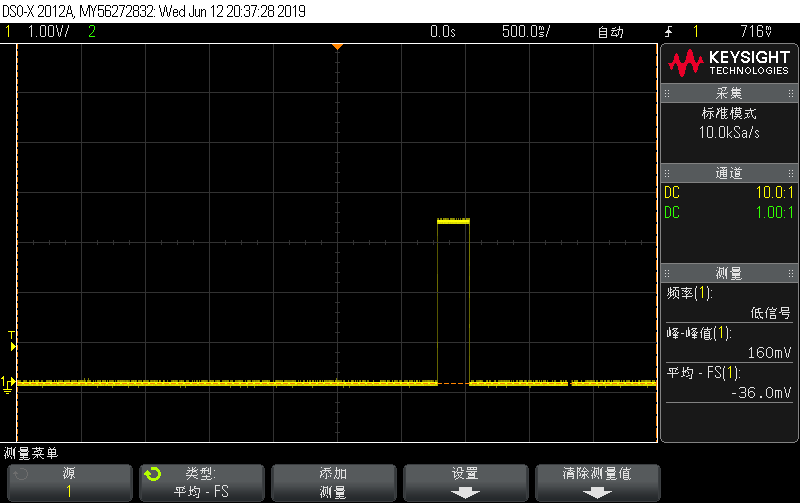
\includegraphics[scale=0.3]{fig/result/module4_result1.png}
        \caption{最终输出波形}
        \label{fig:module4_result1}
    \end{figure}
    
    此时电路的输出电压能满足下一级数字电路的检测要求,但是电路的恢复时间大约为200ms,
    长于仿真时测量的时间。这是因为现实世界中传感器工作状态和仿真时不同而导致的。
    实际传感器输出电压恢复时间比仿真时时间要长,所以最终电路输出波形的实际恢复时间也要长于仿真时间。

    \item 升压斩波电路
    
    我使用的升压斩波电路模块如图\ref{fig:module5}所示:

    \begin{figure}[H]
        \centering
        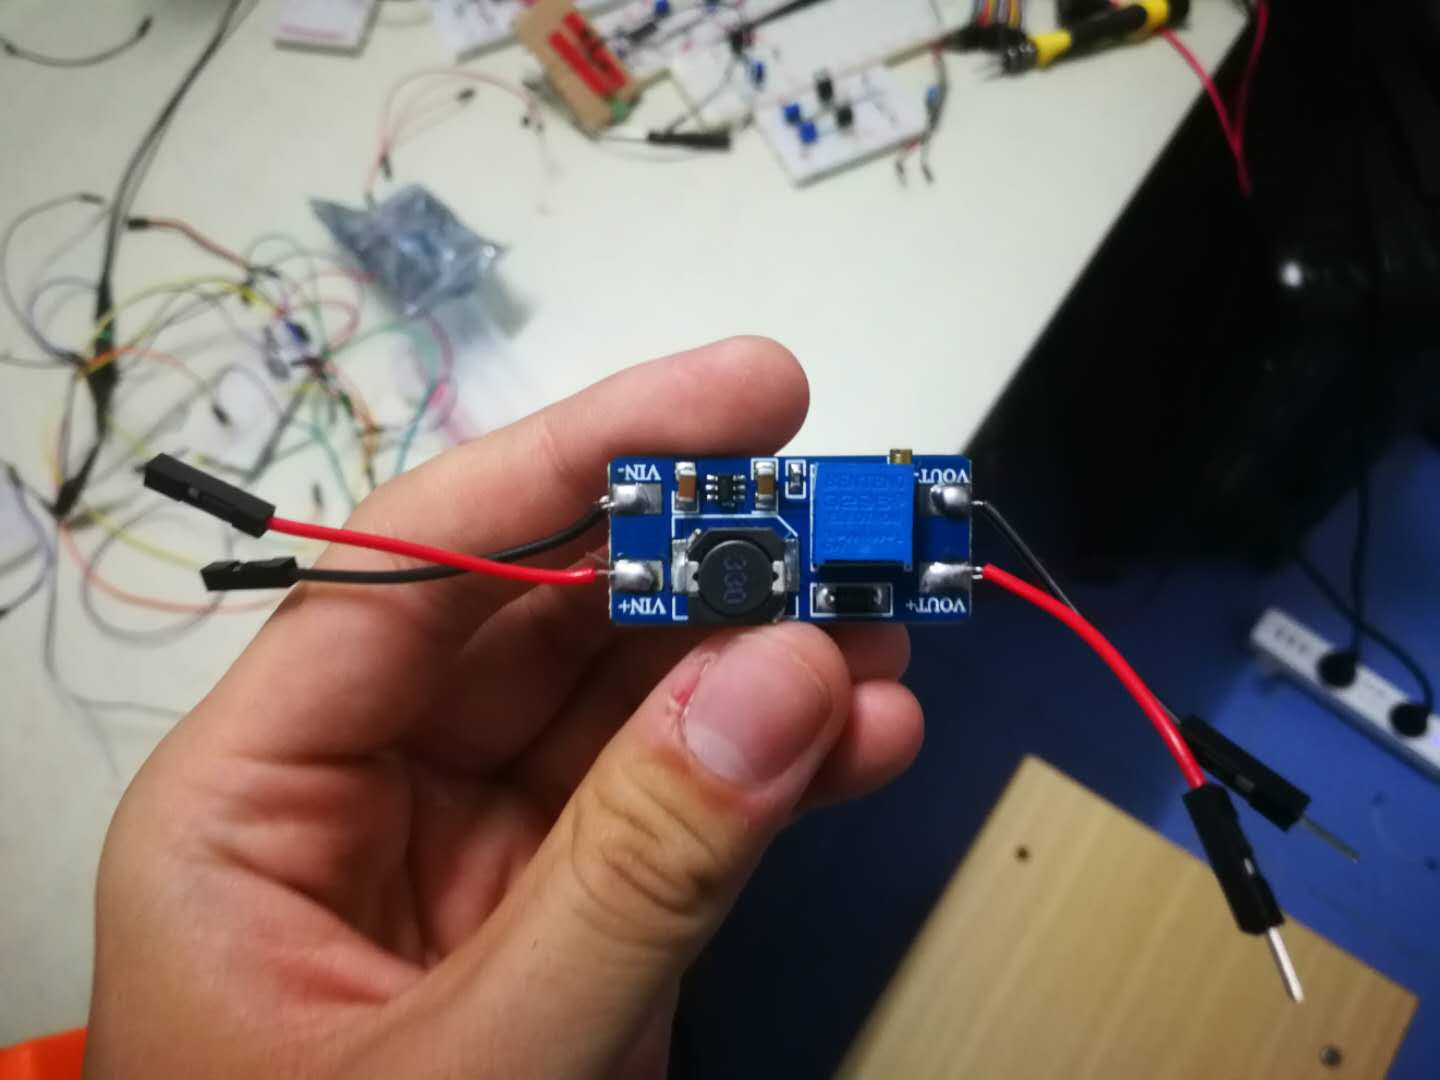
\includegraphics[scale=0.1]{fig/result/module5.png}
        \caption{BOOST电路模块}
        \label{fig:module5}
    \end{figure}
    
    其输出电平波形如图\ref{fig:module5_result1}所示:
    \begin{figure}[H]
        \centering
        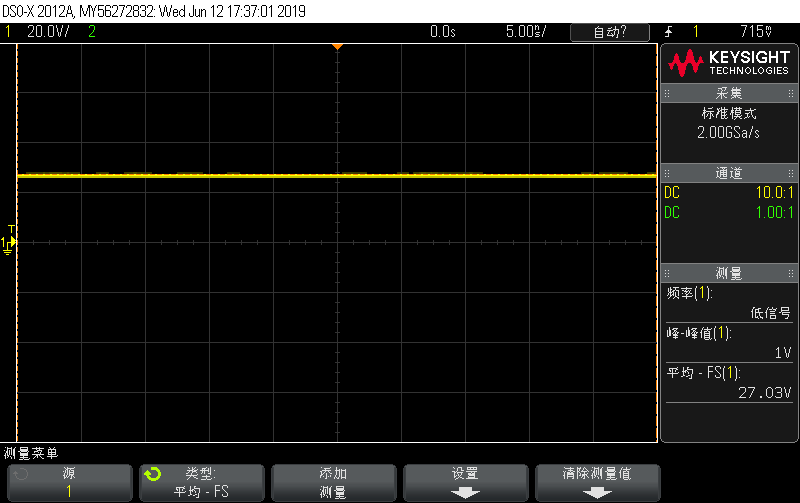
\includegraphics[scale=0.3]{fig/result/module5_result1.png}
        \caption{BOOST电路模块输出波形}
        \label{fig:module5_result1}
    \end{figure}

    其输出电平为27.03V,满足后级电路要求,且经过测试发现其带载能力较强。

\end{enumerate}

    \subsection{数字电路模块}
\begin{enumerate}

    \item Arduino Mega 开发板
    
    我使用的Mega板如图\ref{fig:module6}所示:
    \begin{figure}[H]
        \centering
        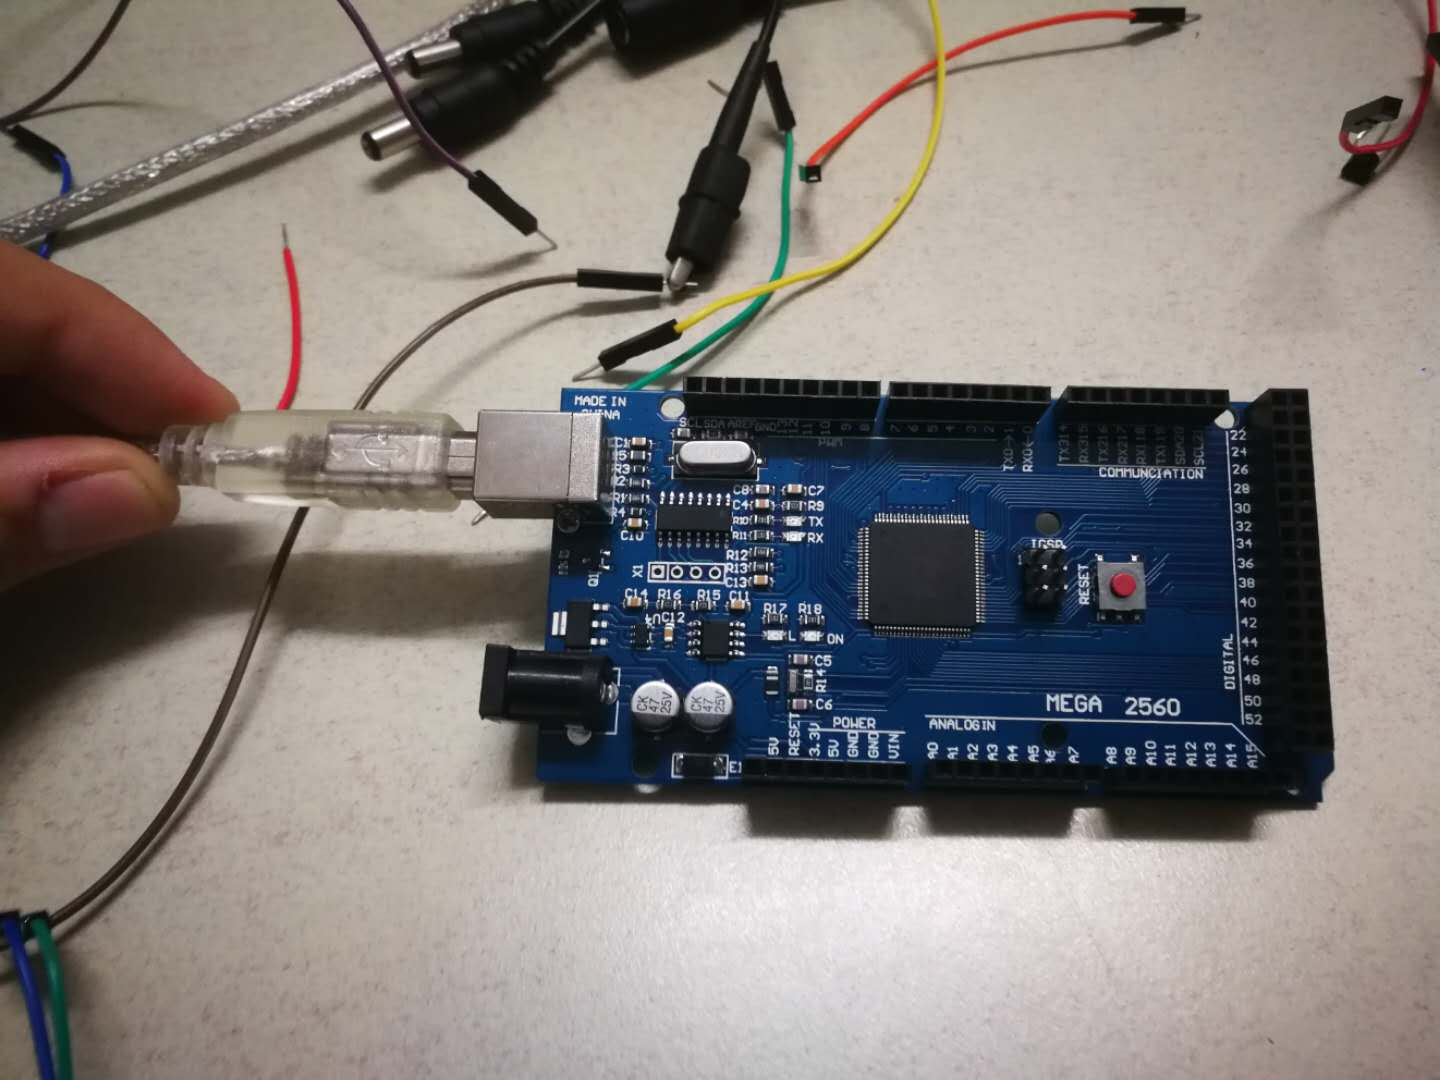
\includegraphics[scale=0.1]{fig/result/module6.png}
        \caption{Arduino Mega开发板}
        \label{fig:module6}
    \end{figure}
    
    其主控代码和连线如下:

\begin{lstlisting}
    /* main.ino */
    #include <stdlib.h> 
    #include <Wire.h>
    #include <LiquidCrystal_I2C.h>
    
    // set the LCD address to 0x20 for a 16 chars and 2 line display
    LiquidCrystal_I2C lcd(0x20,16,2);  
    
    //pin 
    int sensor = A5 ;
    int peopel_pin = 2; 
    int fan_pin = 3;
    
    float temprature;
    float tmp; 
    bool has_people = false ; 
    unsigned long last_time = 0 ;
    
    void setup()
    {
      attachInterrupt(0,toggle_people,RISING);
      pinMode(fan_pin,OUTPUT);
    
      lcd.init();                      // initialize the lcd 
      lcd.backlight();
      
      lcd.home();
      lcd.clear();
    
      lcd.print("init complete");
      delay(2000);
      lcd.clear();
    }
    
    void loop()
    {
      tmp = analogRead(sensor) ;    //read temprature 
      temprature = tmp/2;

      lcd.clear();                  //begin show 
      lcd.setCursor(0,0); 
      lcd.print("temp:");
      lcd.print(temprature);
      lcd.setCursor(0,1);

      if(has_people)
      {
        lcd.print("has people"); 
        if(temprature > 30)
        {
          analogWrite(fan_pin,255); //control fan to max speed 
        }
        else
        {
          analogWrite(fan_pin,180); //control fan to lower speed 
        }
      }
      else 
      {
        lcd.print("no people");
    
        analogWrite(fan_pin,0);     //shutdown fan 
      }
    
      delay(1000);
    }
    
    void toggle_people()            //if detect people in or out
    {
      if(millis()-last_time> 500)   //here set a minimum time to avoid
      {                             //mistake , set at 500 ms 
        has_people = !has_people ; 
      }
    
      last_time = millis();
    }        
\end{lstlisting}

    需要注意的是,我在这里设置了一个500ms的防误触时间,也就是说,如果在500ms内有多次人进出检测范围的情况,则
    主控板只会检测一次。如果为了提升电路检测的实时性,可以适当减少此处的防误触时间。

    \item LCD 显示屏
    
    我使用的LCD显示屏如图\ref{fig:module7}所示:
    \begin{figure}[H]
        \centering
        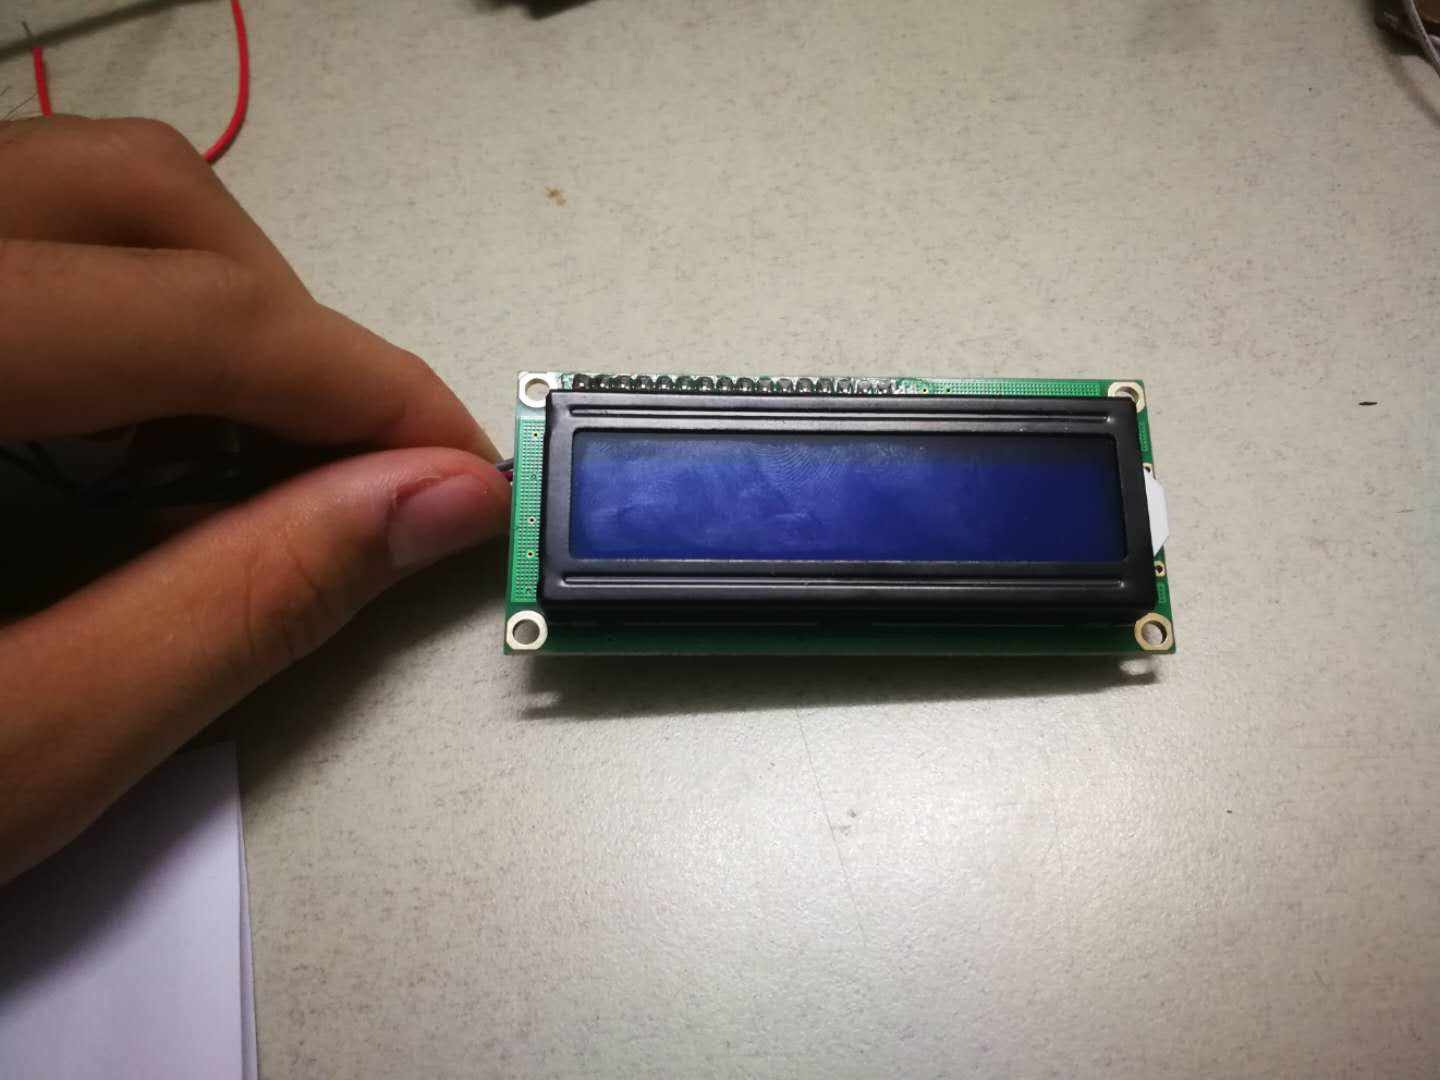
\includegraphics[scale=0.1]{fig/result/module7.png}
        \caption{LCD 显示屏}
        \label{fig:module7}
    \end{figure}

    这是一个只有2行,每行16个字符的显示屏,仅能初步满足显示需求。

    \item L298N 电机驱动模块
    
    我使用的电机驱动模块如图\ref{fig:module8}所示:
    \begin{figure}[H]
        \centering
        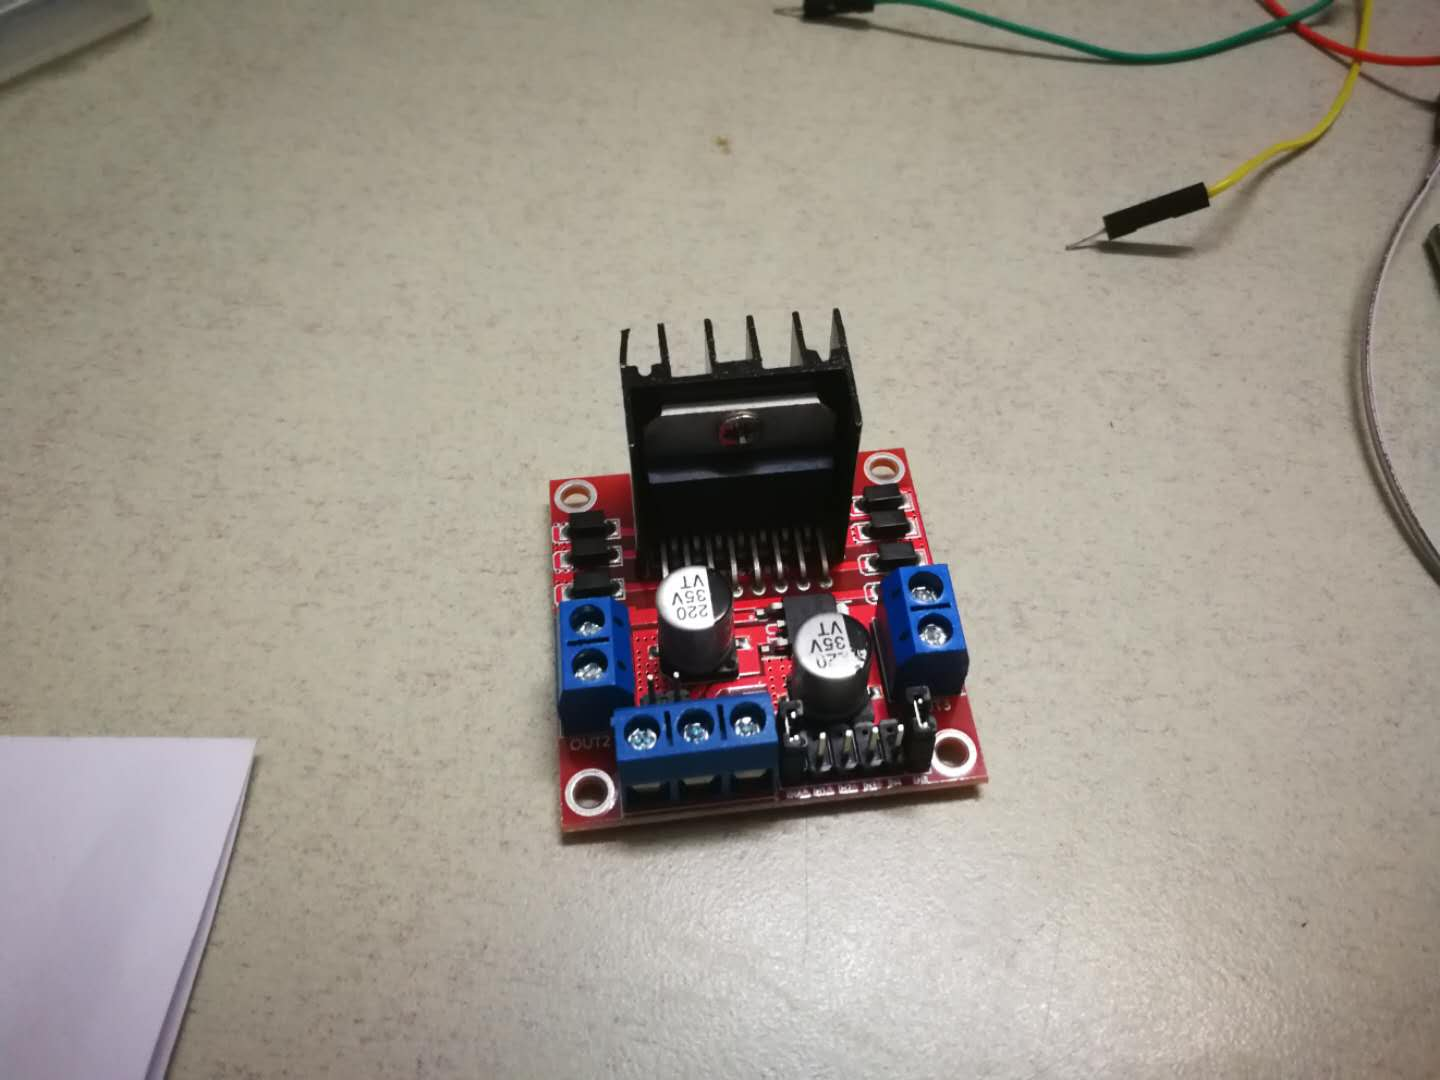
\includegraphics[scale=0.1]{fig/result/module8.png}
        \caption{L298N 电机驱动模块}
        \label{fig:module8}
    \end{figure}

    \item 12V 直流风扇
    
    我使用的12V 直流风扇如图\ref{fig:module9}所示:
    \begin{figure}[H]
        \centering
        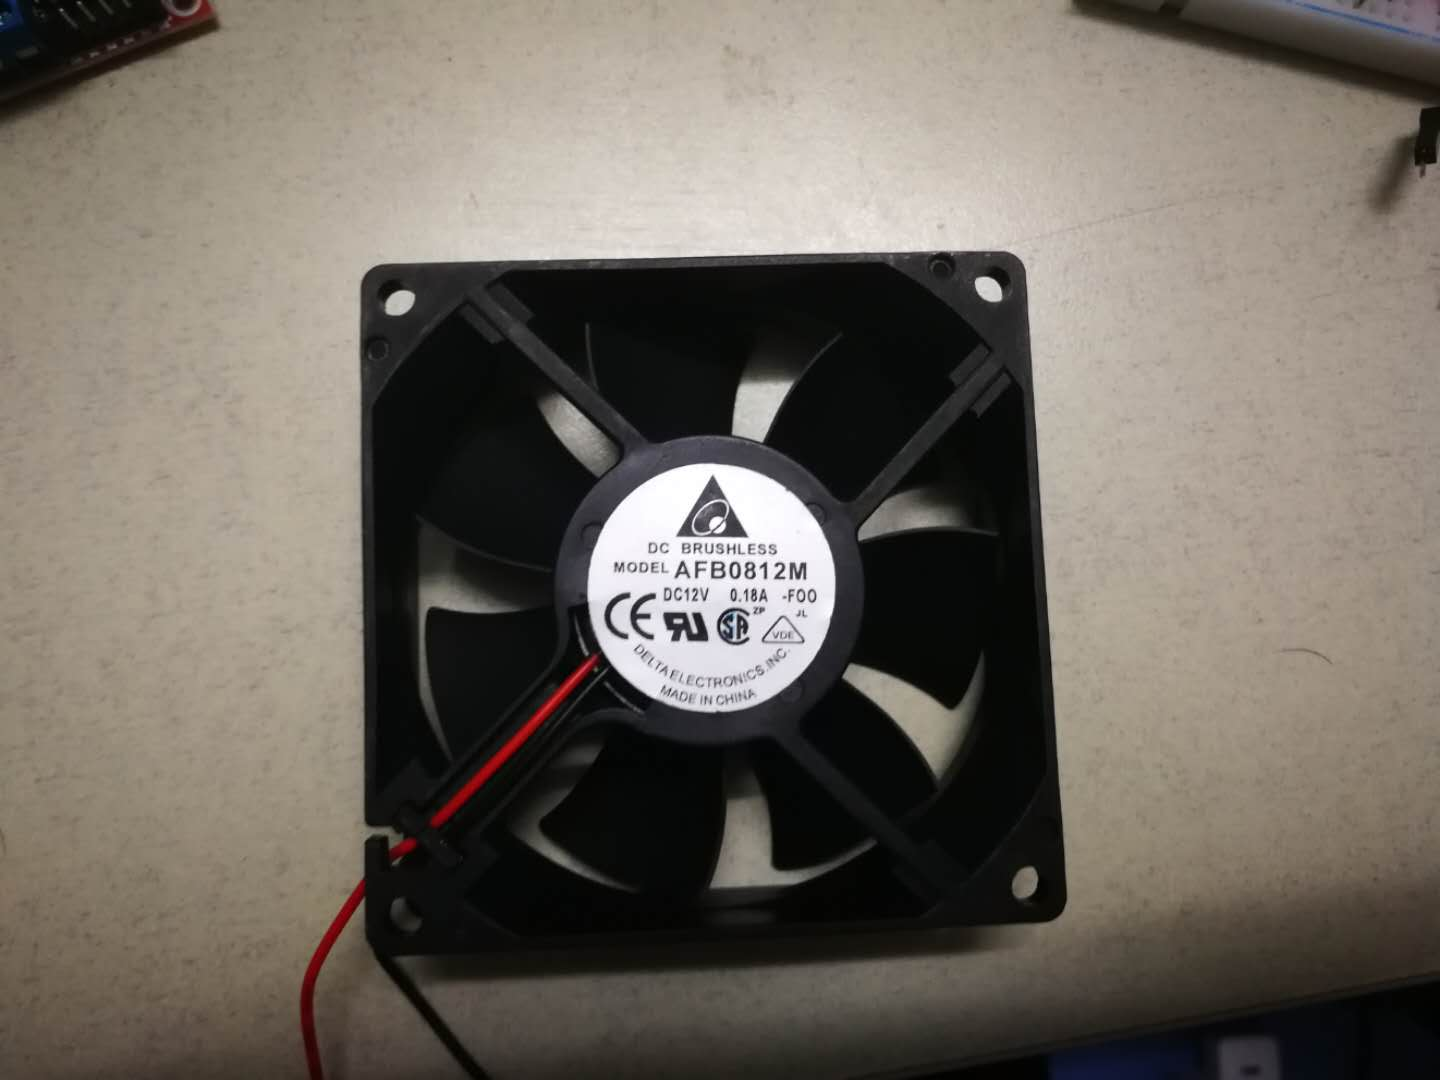
\includegraphics[scale=0.1]{fig/result/module9.png}
        \caption{12V直流风扇}
        \label{fig:module9}
    \end{figure}

    \item 18650 锂电池
    
    我使用的锂电池如图\ref{fig:module10}所示:
    \begin{figure}[H]
        \centering
        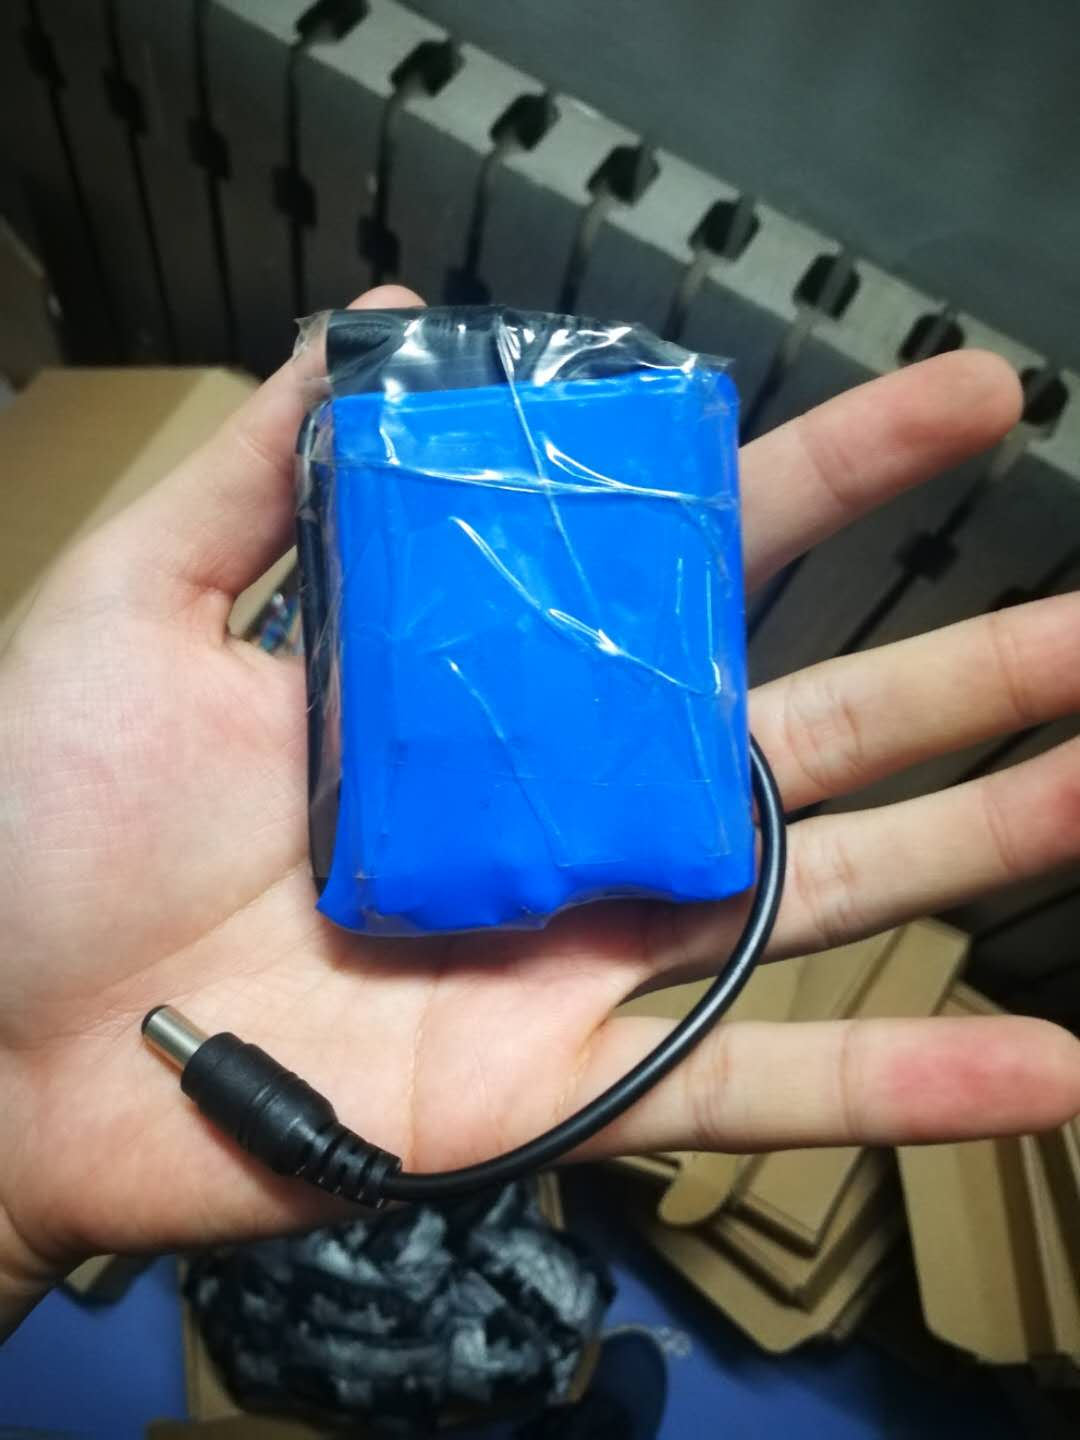
\includegraphics[scale=0.1]{fig/result/module10.png}
        \caption{18650 锂电池}
        \label{fig:module10}
    \end{figure}

    后来由于时间问题,我并没有如预期一样开发一个蓝牙APP,所以在此就并不展示我使用的蓝牙模块了。

    以上模块经过测试都没有问题。

\end{enumerate}

    \subsection{综合调试}

    整体调试电路如图\ref{fig:total}所示:

    \begin{figure}[H]
        \centering
        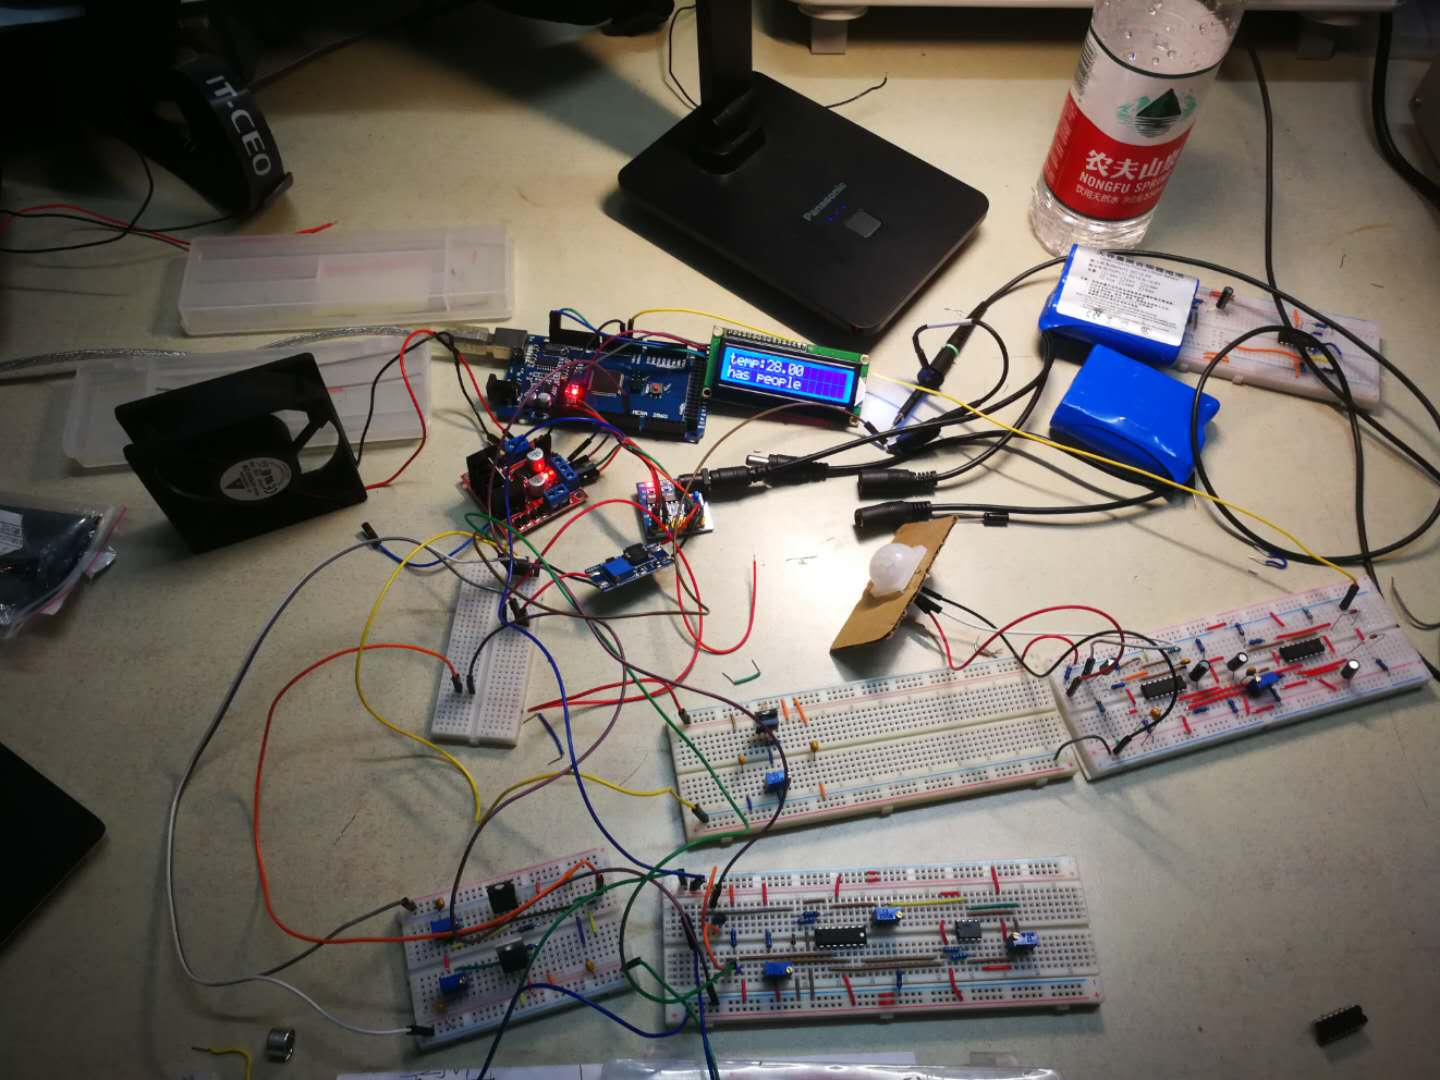
\includegraphics[scale=0.2]{fig/result/total.png}
        \caption{整体调试电路}
        \label{fig:total}
    \end{figure}

    最终测试结果良好,所得展示视频一共有两个:人进出感应范围的视频“people\_in\_out.mp4",以及
    人在范围内不同温度下风扇的转速不同的视频“people\_in\_temp\_rise.mp4",两个视频现都已经放在了“./2-experiment"文件夹下。
    
    (提示,温度和有无人的检测结果可以根据LCD显示屏上的结果来进行判断,
    而对应的风扇转速变化如果不好肉眼观察,可以通过听风扇转动声响来区分。
    当风扇转速实在过慢时,风叶转动会有十分明显的噪声,与正常情况下风扇的无噪声运动十分不同)
    
\section{实验中电路出现的问题以及原因分析}    

这个项目的复杂度,是我在设计之前从未想到的。我在这个过程中,遇到的
主要问题主要有如下几点:

\begin{enumerate}
    \item 前一级输出电流不足的问题
    
    前一级输出电流不足的问题,在电源模块中体现的尤为明显。在正负电源模块中,当我加入后一级电路后,我发现
    前一级电路往往因为输出功率不够(以及后一级输入电阻对前一级电路的影响)的原因,原先调整好的电压又会发生偏移,
    需要重新对进行前一级电路的输出电压调整。
    情况严重时,甚至无法通过调整的方式使得前一级输出电压恢复到期望电压。

    对于这一问题,我通过在前后级电路中间,引入由功放构成的电压跟随器解决了问题。这样一来,
    一方面功放基本可以满足后一级模拟电路的电流需求,
    另一方面,对于前一级电路而言,后一级输入电阻相当于无穷大,降低了对其带载能力的要求。
    所以带载能力的问题成功得到了解决。

    \item 热释电传感器检测范围不足
    
    对于我设计出来的第一版电路,我最终测试所得的比较稳定的检测范围仅仅为5-8cm,这远远低于我项目的使用要求。
    又由于其还存在其他问题(见“4 基本电路模块电路原理/4.1 模拟电路模块/4.热释电测量电路”),
    所以我设计了第二版实验电路,但即使是这样,最终稳定的检测距离也只有20cm左右,
    超出这一范围则会有漏检测和误检测的现象。这样的检测距离,与市面上的被动式热释电传感器7m左右
    的检测范围相差过大。

    经过我调查得知,现在热释电传感器的主流电路实现方案为使用BIS0001运算芯片,基本电路如图\ref{fig:review1}所示。
    
    \begin{figure}[H]
        \centering
        \includegraphics[scale=0.4]{fig/review/1.png}
        \caption{经典热释电传感电路}
        \label{fig:review1}
    \end{figure}

    BIS0001运算芯片内部由多个运放以及一定的数字逻辑电路构成,其电路复杂度比个人的实验电路要复杂得多,所以能实现更为精确的检测精度和更加
    广阔的检测范围也就并不奇怪了。
    
    \item PT1000体积过小,给升温和温度测量带来了很大的麻烦。
    
    在测量PT1000上温度和输出电压之间的关系,以验证电路设计没有问题的过程中,我发现,实验室的PT1000电阻为裸电阻,其体积不足半个指甲盖大,
    这给其上的升温,降温,以及温度检测带来了很大的不便。为了测量其上温度,并且尽量减少对电路的干扰,我从社团处借了一个手持热成像仪,通过主动式红外
    传感来获取PT1000上的近似温度;而为了对它进行升温和降温,由于缺乏实验条件,我只能用手捂和吹气的方式来改变PT1000表面温度,这也给实验带来
    了很大的不便。最终我仅仅获得几组比较有代表性的数据,没能够获得电路输出电平随环境温度的近似变化曲线。

    \item 电源种类过多
    
    这是我本次电路设计中的硬伤。在我最初设计的电路中,由于要使用到正负12V来给运放供电,而整体电路的电源仅为一个12V的锂电池,所以需要使用
    一个正负电源模块。而为了保证正负电源模块正常工作,又需要保证其输入电压大于26V,这就意味着电路中又需要引入一个DC/DC升压模块。
    同时,由于部分电路和传感器(比如主控板Arduino Mega 和 L298N电机驱动模块)需要工作在5V电压下,所以电源管理电路中还需要
    一个12V转5V的电压模块。
    仅仅在电源管理电路中,电路就需要用到3个模拟电路模块:升压斩波电路,正负电源电路以及5V稳压电路模块。

    这样的设计一方面会像上文所述,带来输出功率不足的问题;另一方面,功放和三端稳压器的引入会明显提升电路功耗,
    而这并不是一款便携式电子产品设计所希望看到的。

    所以说,在第二版热释电传感电路的设计中,我就充分考虑到了这个问题。一方面,我将所需要的电源总数减少为1个,也就是说仅仅需要一个5V的电压;
    同时,为了配合这个5V的电压,使得电路能够正常工作,我将所有运放的正极参考电压全部设置为2.5V,通过这样的方式让电路近似的以2.5V作为中间值,
    在2.5V上下进行电压波动。不论是仿真还是实测都证明了这样的电路设计是可行的。

    但是比较遗憾的是,由于时间问题,我没能够将温度传感电路也同样改为只需要5V电压的单电源电路。而从原理上来说,由于温度传感电路中,常用的电压值都在
    0-5V之间,所以温度传感电路是存在被改为单电源电路的可能的。

    这个问题同时也让我理解到并行工程这一思想的重要性,不仅在设计电源时要考虑到各个电路模块的需求,
    也需要在设计电路模块时,减少所需要电源种类并降低对于电源质量的要求。
    这样一来,通过电路模块之间的相互配合来降低电路复杂度,提升电路工作性能。

\end{enumerate}

同时,由于时间关系,整个项目比较遗憾的包括:

\begin{enumerate}
    \item 没有减少电源种类,使得现在的电源管理模块数量过多
    \item 超出课程所学范围的升压斩波电路并没有自己搭建,并研究一下其工作原理和实际工作特性。
    \item 由于Arduino Mega ADC芯片的精度,最终只能实现精度为0.5$^{\circ} C$的温度测量
    \item Multisim没能够使用支电路的方式,进行一次整体电路仿真
    \item 没能够在调试完整体电路以后,用Altium Designer画一块双层PCB板来简化电路连线
    \item 没有足够的时间来实现自己原本想要编写的手机端APP
    \item 所使用的显示屏过于简单,缺少进一步的人机互动
\end{enumerate}

\section{项目的改进方向}

项目下一步的改进方向包括有:

    \subsection{模拟电路部分}

    \begin{enumerate}
        \item 对于热释电传感器,可以尝试使用BIS0001芯片进行更高层次的模拟电路设计,以此来进一步提升热释电传感的检测精度
        \item 对于温度检测电路,在电桥电路处使用恒流源电路来将PT1000阻值变化直接转变为电信号,从而省去
        近似估算的过程,提高电路检测的精确度。
        
        同时,考虑使用在淘宝上有售卖的更大一些的PT1000探头而不是PT1000裸电阻。这样一来,一方面是方便测试其PT1000表面温度,
        另一方面也方便将其和电路隔离开来,单独对其进行加热降温等操作,从而获得更大的温度变化范围,
        能够更加准确的验证输出电压和PT1000表面温度之间的关系。

        除此以外,将双电源改为单电源供电也应该是下一步改进的方向之一。

        最后,可以考虑使用差分放大芯片代替精密运放以实现电路的差分放大。但是我并不确定这样做能够提升检测精度,
        只能说可以将其仅仅作为一个改进的尝试方向。

        \item 对于电源管理电路,一方面,应该尽可能的减少所使用的电源种类,这样一来既可以减少功放管的使用,又可以降低
        电路功耗。

    \end{enumerate}

    \subsection{数字电路部分}

    \begin{enumerate}
        \item 对于主控板,由于在实验过程中,Arduino上的ADC芯片精度不够,导致最终温度的可识别精度也只有0.5摄氏度。为了进一步提升温度检测的准确度
        除了在模拟电路部分进一步做电路改进以外,也应该考虑在主控板上外接一个精度更高的AD采集模块(比如16位AD采集模块),或者更换Arduino控制板
        为STMF407开发板(前者使用的是一块10位AD模块,后者使用的是一块12位逐次逼近型AD转换模块)。

        \item 更换LCD显示屏。可以更换其为更大的LCD显示屏甚至是触摸屏,增强与用户之间的互动性。
        
        \item 开发蓝牙移动端APP,让用户可以通过手机直接操控风扇
    
    \end{enumerate}

\end{spacing}
\end{document}